\documentclass[aspectratio=169]{beamer}  
\usefonttheme{professionalfonts}
\usepackage{xeCJK}
\usepackage{fontspec}
\usepackage{graphicx}
\usepackage{listings}
\usepackage{xcolor}
\usepackage{indentfirst}
\usepackage{tikz}
\usepackage{amssymb}
\usepackage{amsthm}
\usepackage{amsmath}
\usepackage{tabularx}
\usepackage{hyperref}
\usepackage{comment}
\usepackage{ulem}
\usepackage{version}
\usepackage{thmtools}
\usepackage{qtree}
\usepackage{algpseudocode}
\usepackage{mathtools}
\usepackage{multicol}
\usepackage{xcolor}
\usepackage{diagbox}

\usefonttheme[onlymath]{serif}

\XeTeXlinebreaklocale "zh"
\XeTeXlinebreakskip = 0pt plus 1pt

\setsansfont{JetBrainsMono-Medium.ttf}
\setCJKmainfont[AutoFakeBold,AutoFakeSlant]{NotoSansTC-Regular.otf}
\usetikzlibrary{arrows,decorations.markings,decorations.pathreplacing}
\newenvironment{Hint}{\noindent\textbf{Hint.}}{}

\tikzstyle {graph node} = [circle, draw, minimum width=1cm]
\tikzset{edge/.style = {decoration={markings,mark=at position 1 with %
            {\arrow[scale=2,>=stealth]{>}}},postaction={decorate}}}

\lstset{
    language=C++,
    basicstyle=\ttfamily\tiny,
    numberstyle=\tiny,
    numbers=left,
    stepnumber=1,
    numbersep=3pt,
    commentstyle=\color{black!50},
    keywordstyle=\color{white!0!blue},
    stringstyle=\color{black!50!green},
    showspaces=false,
    showstringspaces=false,
    showtabs=false,
    tabsize=4,
    captionpos=b,
    breaklines=true,
    breakatwhitespace=false,
    escapeinside={\%*}{*)},
    morekeywords={*}
}

\AtBeginSection[]{
  \begin{frame}
  \vfill
  \centering
  \begin{beamercolorbox}[sep=8pt,center,shadow=true,rounded=true]{title}
    \usebeamerfont{title}\insertsectionhead\par%
  \end{beamercolorbox}
  \vfill
  \end{frame}
}

\title{Basic Graph Algorithms}
\author{zhu \& sam571128}
\date[師大附中暑期培訓]

\usetheme{Madrid}
\usecolortheme{default}
\setbeamertemplate{itemize items}[square]
\setbeamertemplate{enumerate items}[default]
\setbeamertemplate{blocks}[default]

\begin{document}

    %title
    \begin{frame}
        \titlepage
    \end{frame}
    
    %contents
    \begin{frame}{這兩天會教的東西}
        \begin{itemize}
            \item 圖的儲存
            \item 圖的遍歷
            \item 歐拉迴路、哈密頓迴路
            \item 拓樸排序
            \item 最短路徑
            \item 樹論
            \begin{enumerate}
                \item 性質
                \item 樹直徑、樹重心
                \item 樹壓平
                \item 樹 dp、換根 dp
            \end{enumerate}
            \item 並查集
            \item 最低共同祖先
            \item 最小生成樹
        \end{itemize}
    \end{frame}
    \begin{frame}{owo}
        \begin{center}
            今天簡報上面所有題目的 code 我都放到 \href{https://github.com/Iambamzhuuuu/Basic-Graph-Algorithm}{github} 上了\\
            如果不會寫的話可以去參考 ><
        \end{center}
    \end{frame}
    %ready
    \begin{frame}{圖是甚麼?}
        \begin{itemize}
            \item 圖$G$是一個由點集$V$和邊集$E$所構成的結構 $G=(V,E)$\\
        \end{itemize}
        \vspace{2mm}
        \begin{center}
            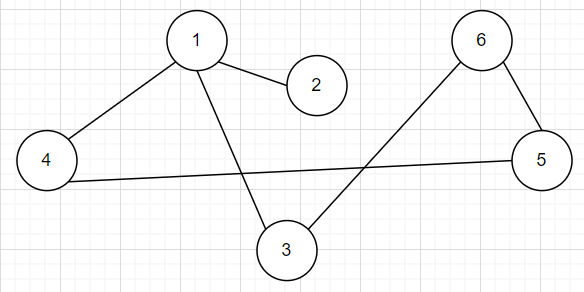
\includegraphics[scale=0.5]{images/graph.png}
        \end{center}
    \end{frame}
    
    \begin{frame}{名詞解釋}
        \begin{itemize}
            \item 圖 (Graph)
            \item 點 (Vertex) / 邊 (Edge)
            \item 有向圖 (Directed Graph) / 無向圖 (Undirected Graph)
            \item 權重 (Weight)
            \item 點度 (Degree)
            \item 環 (Cycle) / 迴路 (Circuit)
        \end{itemize}
    \end{frame}
    
    \begin{frame}{名詞解釋}
        \begin{itemize}
            \item 連通的 (Connected)
            \item 連通分量 / 連通塊 (Connected Components)
            \item 相鄰 (Adjacent): 鄰邊 (Adjacent Edge) / 鄰點 (Adjacent Vertex)
            \item 自環 (Self Loop) / 重邊 (Multiple Edge)
            \item 簡單圖 (Simple Graph) / 簡單路徑 (Simple Path)
        \end{itemize}
    \end{frame}
    
    \begin{frame}{特別的圖}
        \begin{itemize}
            \item 樹 (Tree): 包含星星 (Star)、鍊 (Chain)
            \item 有向無環圖 DAG (Directed Acylic Graph)
            \item Functional Graph: 每個點的出度都是 $1$ 的有向圖
            \item 二分圖 (Bipartite Graph): 可以被塗成兩種顏色且相同顏色不相鄰的圖
        \end{itemize}
    \end{frame}
    
    %rready
    \begin{frame}{熱身一下}
        \begin{itemize}
            \item 笨笨國國王給你$n$個資訊,告訴你有一條一公里的路徑可以讓你從$a$通向$b$
            \item<2-> 笨竹 想要$O(1)$知道他是否可以走一公里就從$u$到達$v$
            \item<3-> 這樣的話,你會想怎麼存資訊?
            \item<4-> 聰明的你一定想到了 > <
        \end{itemize}
    \end{frame}
    
    %start
    %1
    \section{圖的儲存}
    
    \begin{frame}{鄰接矩陣 (Adjacency Matrix)}
    \begin{columns}
    \begin{column}{0.6\textwidth}
        \begin{itemize}
            \item 對於一張圖,我們用鄰接矩陣 $A$ 儲存
            \item $A[i][j]$會存$i$到$j$的邊的資訊,例如權重或是是否有這條邊
            \item 在無向圖當中,$A[i][j]$ 會等於 $A[j][i]$
            \item 可以在 $O(1)$ 查詢 $i,j$ 之間的邊的資訊
            \item 在遍歷時,要枚舉所有點,複雜度較差
        \end{itemize}
    \end{column}
    \begin{column}{0.4\textwidth}
        \begin{center}
            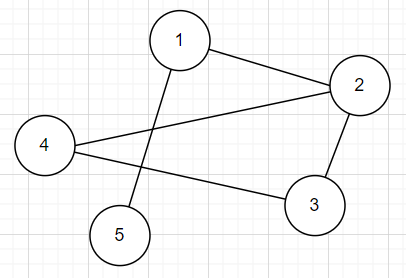
\includegraphics[scale=0.3]{images/Adjacency Matrix.png}
        \end{center}
        \begin{center}
        \begin{tabular}{|c|c|c|c|c|c|}
            \hline
                  & $1$ & $2$ & $3$ & $4$ & $5$  \\ \hline 
             $1$  &  -  & $1$ & $0$ & $0$ & $1$  \\ \hline
             $2$  & $1$ &  -  & $1$ & $1$ & $0$   \\ \hline
             $3$  & $0$ & $1$ &  -  & $1$ & $0$  \\ \hline
             $4$  & $0$ & $1$ & $1$ &  -  & $0$  \\ \hline
             $5$  & $1$ & $0$ & $0$ & $0$ &  -  \\ \hline
        \end{tabular}
        \end{center}
    \end{column}
    \end{columns}
    \end{frame}
    
    \begin{frame}{鄰接串列 (Adjacency List)}
    \begin{columns}
    \begin{column}{0.6\textwidth}
        \begin{itemize}
            \item 我們可以開$|V|$個vector,用來存節點$i$的鄰邊資訊
            \item 它的優點是可以節省空間
            \item 犧牲了 $O(1)$ 查詢邊的優點,換取空間
            \item 在遍歷時,只需要跑過相鄰的點,複雜度較好
        \end{itemize}
    \end{column}
    \begin{column}{0.4\textwidth}
        \begin{center}
            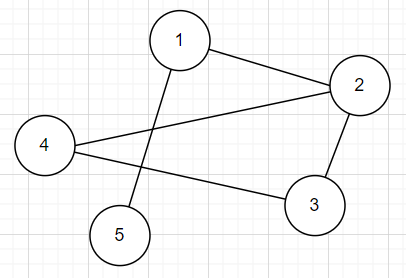
\includegraphics[scale=0.3]{images/Adjacency Matrix.png}
        \end{center}
        \begin{center}
        \begin{tabular}{|c|c|}
                                \hline
            $V$ &  $A[V]$    \\ \hline
            $1$ &  $2, 5$    \\ \hline
            $2$ &  $1, 3, 4$ \\ \hline
            $3$ &  $2, 4$    \\ \hline
            $4$ &  $2, 3$    \\ \hline
            $5$ &  $1$       \\ \hline
        \end{tabular}
        \end{center}
    \end{column}
    \end{columns}
    \end{frame}
    
    %2
    \section{圖的遍歷}
    \begin{frame}{圖的遍歷 (Traversal)}
        \begin{itemize}
            \item 就是把整張圖走一遍
            \item 在這裡介紹 BFS 跟 DFS 兩種走訪方式
            \item<2-> 不同的走訪方式或順序會有不同的效果
        \end{itemize}
    \end{frame}
    %BFS
    \begin{frame}{廣度優先搜尋 (Breadth First Search)}
        \begin{itemize}
            \item BFS 會優先走訪自己的鄰點
            \item<2-> 實作上我們會開一個 queue,用來維護接下來要走的點
            \item<3-> 要做的事情是把 queue 最前面的點拿出來,將他的鄰點中沒走過的推進 queue
            \item<4-> 時間複雜度:$O(|V|+|E|)$
        \end{itemize}
    \end{frame}
    \begin{frame}{廣度優先搜尋 (Breadth First Search)}
        \begin{columns}
            \begin{column}{0.5\textwidth}
                \begin{center}
                    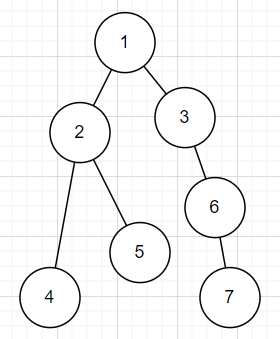
\includegraphics[scale=0.5]{images/BFS.png}
                \end{center}
            \end{column}
            \begin{column}{0.5\textwidth}
                \begin{enumerate}
                    \item \texttt{push} $1$, $\mathtt{queue} = \{1\}$ 
                    \item \texttt{pop} $1$ , $\mathtt{queue} = \{2,3\}$
                    \item \texttt{pop} $2$ , $\mathtt{queue} = \{3,4,5\}$
                    \item \texttt{pop} $3$ , $\mathtt{queue} = \{4,5,6\}$
                    \item \texttt{pop} $4$ , $\mathtt{queue} = \{5,6\}$
                    \item \texttt{pop} $5$ , $\mathtt{queue} = \{6\}$
                    \item \texttt{pop} $6$ , $\mathtt{queue} = \{7\}$
                \end{enumerate}
            \end{column}
        \end{columns}
    \end{frame}
    
    
    \begin{frame}{BFS CODE}
        \begin{center}
            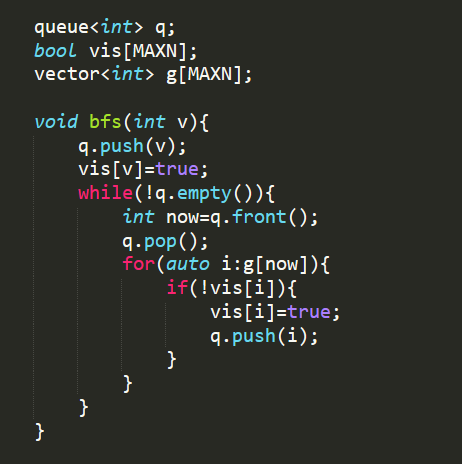
\includegraphics[scale=0.7]{code/bfs_code.png}
        \end{center}
    \end{frame}
    
    
    \begin{frame}{深度優先搜尋 (Depth First Search)}
        \begin{itemize}
            \item DFS 會優先往深的地方走,概念上與 BFS 相似,但改用 stack
            \item 實作的時候我們會用遞迴往能走的點走,若沒有可走的點就回到上一個點
            \item 時間複雜度:$O(|V|+|E|)$
        \end{itemize}
    \end{frame}
    
    \begin{frame}{深度優先搜尋 (Depth First Search)}
        \begin{columns}
            \begin{column}{0.5\textwidth}
                \begin{center}
                    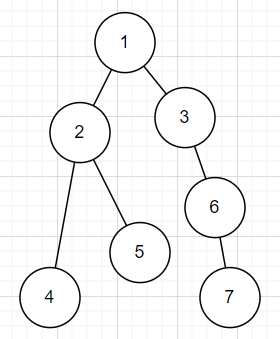
\includegraphics[scale=0.5]{images/BFS.png}
                \end{center}
            \end{column}
            \begin{column}{0.5\textwidth}
                \begin{enumerate}
                    \item \texttt{dfs} $1$, \texttt{stack = \{2,3\}}
                    \item \texttt{dfs} $2$, \texttt{stack = \{4,5,3\}}
                    \item \texttt{dfs} $4$, \texttt{stack = \{5,3\}}
                    \item \texttt{dfs} $5$, \texttt{stack = \{3\}}
                    \item \texttt{dfs} $3$, \texttt{stack = \{6\}}
                    \item \texttt{dfs} $6$, \texttt{stack = \{7\}}
                    \item \texttt{dfs} $7$
                \end{enumerate}
            \end{column}
        \end{columns}
    \end{frame}
    
    \begin{frame}{DFS CODE}
        \begin{center}
            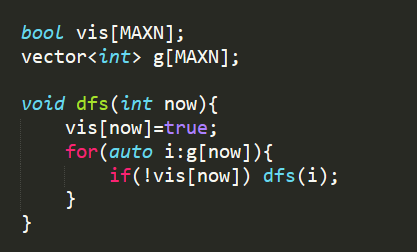
\includegraphics[scale=0.7]{code/dfs_code.png}
        \end{center}
    \end{frame}
    
    %practice
    \begin{frame}{這是一些很裸很裸的題目 ><}
        \begin{block}{\href{https://cses.fi/problemset/task/1192}{CSES Counting Rooms}}
        給一個$n\times m$的地圖,'.'代表地板,'\#'代表牆壁,問你有幾間房間
        \end{block}
        \begin{block}{\href{https://cses.fi/problemset/task/1193}{CSES Labyrinth}}
        給一個$n\times m$的地圖,'.'代表地板,'\#'代表牆壁,'A'代表起點,'B'代表終點,問是否可以從 A 走到 B,若可以則輸出路徑長並且回溯路徑
        \end{block}
    \end{frame}
    \begin{frame}{喵喵喵喵喵}
        \begin{center}
            現在來看一些可以寫的例題 ><
        \end{center}
    \end{frame}
    \begin{frame}{Practice}
        \begin{block}{\href{https://cses.fi/problemset/task/1678}{CSES Round Trip II}}
        給你一張有向圖,判斷這張圖是否有環,如果有環,輸出這個環
        \end{block} 
        \begin{itemize}
            \item<2-> 當 DFS 到這個點時,我們會說走進了這個點
            \item<2-> 當 DFS return 的時候,我們會說離開了這個點
            \item<3-> 可以發現到,如果 DFS 到的這個點的鄰點中,有走進但還沒離開的點,就代表有環
            \item<4-> 實作上可以使用 stack 維護走進但還沒離開的點
            \item<4-> 進入時,將點 push 進去。離開時,將點 pop 掉
            \item<5-> 當找到環後,從 stack 上還原出環上的點
            % 之後補 code
        \end{itemize}
    \end{frame}
    
    \begin{frame}{Practice}
        \begin{block}{\href{https://tioj.ck.tp.edu.tw/problems/1209}{TIOJ 1209 圖論之 二分圖測試}}
        給你一張圖,問它是否為二分圖
        \end{block}
        \begin{itemize}
            \item<2-> 在 DFS 的時候我們可以對它塗顏色
            \item<3-> 塗完 $u$ 時,若相鄰的點中有和 $u$ 相同的顏色,表示它不是二分圖
            \item<4-> 否則當 DFS 完所有連通塊後,都還沒有矛盾,表示它是一張二分圖
        \end{itemize}
    \end{frame}
    
    \section{歐拉迴路、哈密頓迴路}
    \begin{frame}{歐拉迴路 (Eulerian Circuit)}
        \begin{itemize}
            \item 常說的「一筆畫問題」
            \item 歐拉迴路 (Eulerian Circuit):不重複的走過所有邊,並回到原點
            \item 歐拉路徑 (Eulerian Path):從某個點開始,不重複的走過所有邊
            \item 中國郵差問題 (Chinese Postman Problem):找到最短的歐拉迴路
        \end{itemize}
    \end{frame}
    
    \begin{frame}{判斷一張圖是不是有歐拉路徑}
        \begin{itemize}
            \item 沒有奇數度數的節點: 存在歐拉迴路
            \item $2$ 個奇數度數的節點: 存在歐拉路徑
            \item $>2$ 個奇數度數的節點: 不可能一筆畫畫完
        \end{itemize}
        \begin{center}
            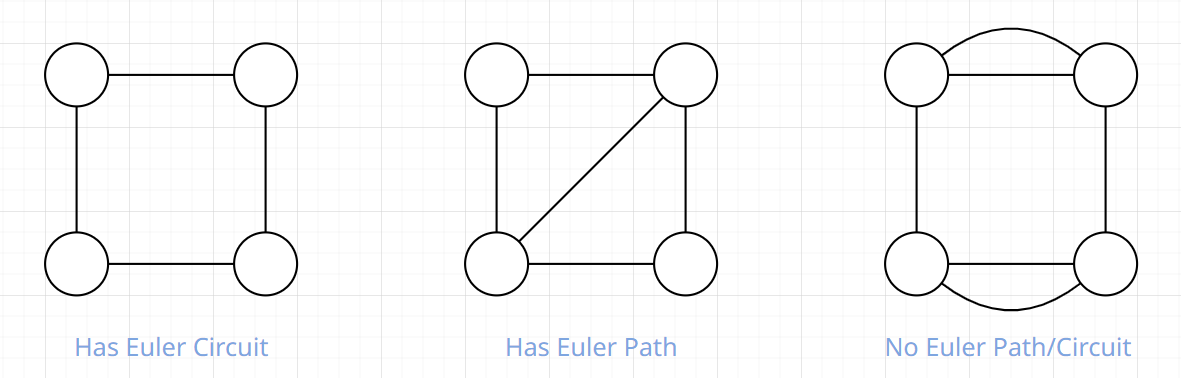
\includegraphics[width=\textwidth]{images/eulerian_graph.png}
        \end{center}
    \end{frame}
    
    \begin{frame}{找到一個歐拉路徑}
        \begin{itemize}
            \item 沒有奇數度數的節點: 任選一個點開始走不重複的邊
            \item $2$ 個奇數度數的節點: 從其中一個奇數度數的點開始走不重複的邊
        \end{itemize}
        \begin{center}
            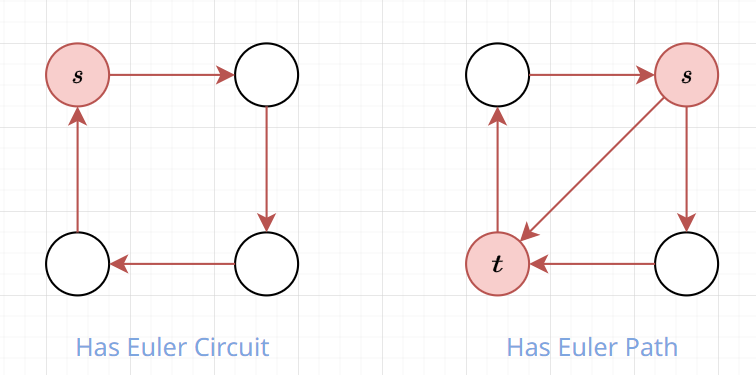
\includegraphics[scale=0.5]{images/euler_path.png}
        \end{center}
    \end{frame}
    
    \begin{frame}{N 筆畫問題}
        \begin{itemize}
            \item 給你一張圖,問最少要幾筆畫才能畫完
            \item $\max(\dfrac{O}{2}, \ 1)$  ($O$ 是奇數度數節點數量)
        \end{itemize}
        \begin{center}
            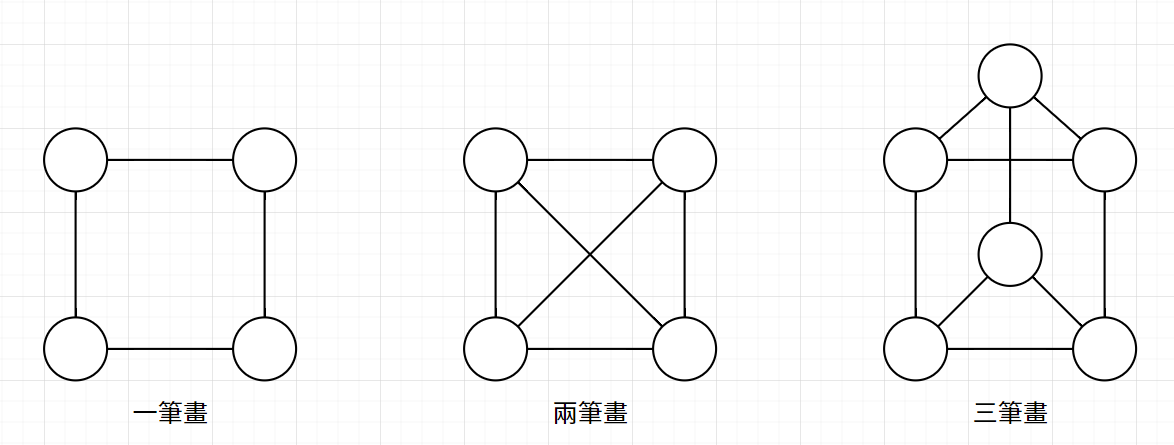
\includegraphics[width=\textwidth]{images/euler_path_2.png}
        \end{center}
    \end{frame}
    
    \begin{frame}{這是一題裸題 ><}
        \begin{block}{\href{https://tioj.ck.tp.edu.tw/problems/1084}{TIOJ 1084 一筆畫問題}}
        給你一張圖,輸出這張圖的一筆畫路徑。
        \end{block}
    \end{frame}
    
    \begin{frame}{Practice}
        \begin{block}{\href{https://tioj.ck.tp.edu.tw/problems/2171}{TIOJ 2171 打卡遊戲}}
        給你一張 $A+B$ 個點,$K$ 條邊的圖,問你一共要幾筆畫可以畫完這張圖
        \end{block}
    \end{frame}
    
    \begin{frame}{哈密頓迴路 (Hamilton Circuit)}
        \begin{itemize}
            \item 哈密頓迴路 (Eulerian Circuit):不重複的走過所有點,並回到原點
            \item 哈密頓路徑 (Eulerian Path):從某個點開始,不重複的走過所有點
            \item 旅行推銷員問題 (Travelling Salesman Problem):找到最短的哈密頓迴路
            \item 可以使用位元 DP 計算答案,但這裡不會講
        \end{itemize}
        \begin{center}
            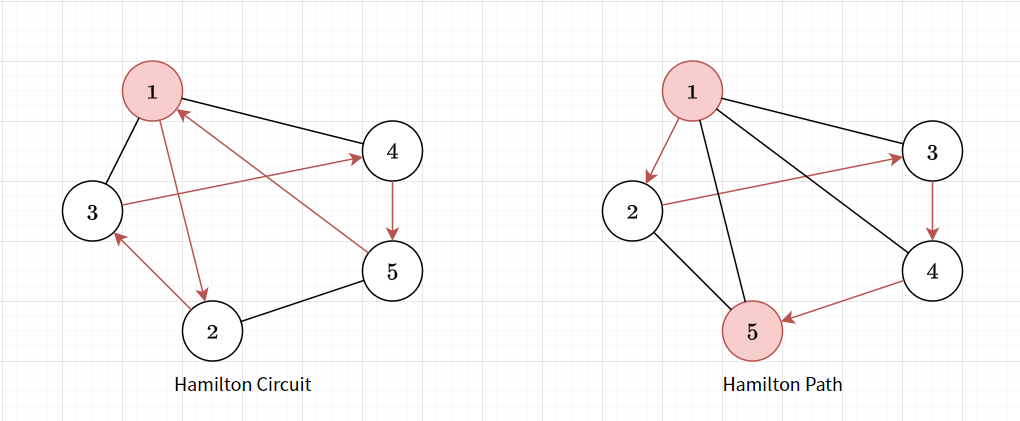
\includegraphics[scale=0.4]{images/hamilton_circuit.png}
        \end{center}
    \end{frame}
    
    \section{拓樸排序 (Topological Sort)}
    
    \begin{frame}{拓樸排序 (Topological Sort)}
        \begin{itemize}
            \item 對於一張 DAG,我們可以找到一個順序
            \item 使得邊只會從前面的點連到後面的點
        \end{itemize}
        \begin{center}
            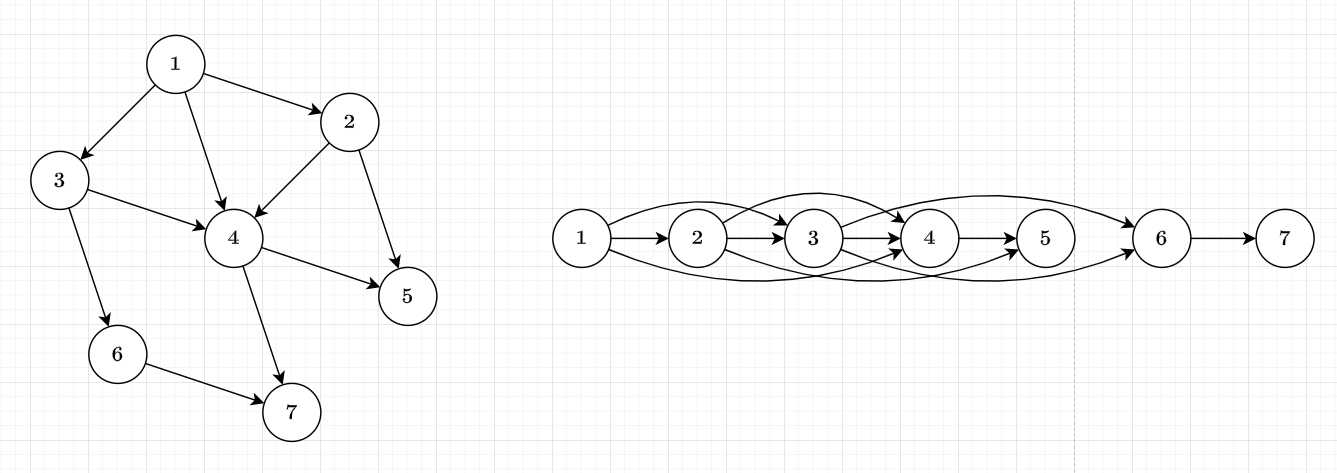
\includegraphics[scale=0.4]{images/topological sort.png}
        \end{center}
    \end{frame}
    
    \begin{frame}{拓樸排序 (Topological Sort)}
        \begin{itemize}
            \item DAG 上至少會有一個入度為 $0$ 的點
            \item<2-> 如果有一個點它的入度不為$0$,那就代表他要先走過前面的點
            \item<3-> 所以我們的起點一定是入度為$0$的點
        \end{itemize}
    \end{frame}
    
    \begin{frame}{拓樸排序 (Topological Sort) 實作}
        \begin{columns}
            \begin{column}{0.65\textwidth}
                \begin{itemize}
                    \item 我們可以開一個陣列 $\texttt{indeg[v]}$ 表示節點$v$的入度
                    \item<2-> 再開一個 queue 把$\texttt{indeg[v]=0}$的節點推進去
                    \item<3-> 取出 queue 最前面的點$u$,把它加進拓樸排序裡面
                    \item<3-> 把$u$和它的出邊拔掉
                    \item<4-> 再去檢查有沒有入度為$0$的點,把它推進 queue
                    \item<5-> 重複做最後就會找到拓樸排序
                \end{itemize}
            \end{column}
            \begin{column}{0.4\textwidth}
                \begin{center}
                    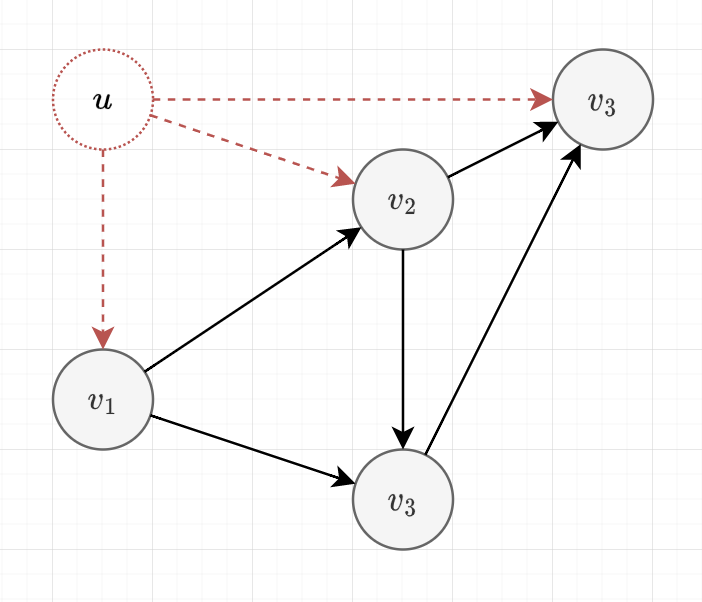
\includegraphics[scale=0.25]{images/topo_bfs.png}
                \end{center}
            \end{column}
        \end{columns}
    \end{frame}
    
    \begin{frame}{拓樸排序 (Topological Sort) Code}
        \begin{center}
            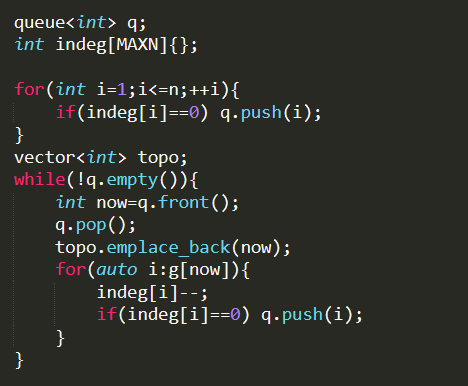
\includegraphics[scale=0.7]{code/topo_code.png}
        \end{center}
    \end{frame}
    
    \begin{frame}{Practice}
        \begin{block}{\href{https://codeforces.com/problemset/problem/510/C}{Codeforces 510C Fox and Names}}
        給你一些照某個奇怪字典序排好的字串,找到字母在字典序的順序。
        \end{block}
    \end{frame}
    
    \begin{frame}{DAG 上 DP (DP on DAG)}
        \begin{itemize}
            \item 在做拓樸排序時,順便轉移 DP 式
            \item 我們來看個例子吧 ><
        \end{itemize}
    \end{frame}
    
    \begin{frame}{Practice}
        \begin{block}{\href{https://cses.fi/problemset/task/1681/}{CSES Game Routes}}
        給你一張 DAG,問你從 $1$ 走到 $n$ 有幾種不同路徑。
        \end{block}
    \end{frame}
    
    \section{最短路徑 (Shortest Path)}
    
    \begin{frame}{最短路徑的東東}
        \begin{itemize}
            \item 單點源最短路徑 (Single Source Shortest Path)
                \begin{itemize}
                    \item BFS (在圖的邊權都是 $1$ 時)
                    \item Dijkstra (在圖的邊權是非負時)
                    \item 0-1 BFS (在圖的邊權只有 $0/1$ 時)
                    \item Bellman-Ford / SPFA (都可以,也可以判斷負環)
                \end{itemize}
            \item 全點對最短路徑 (All Pairs Shortest Path)
                \begin{itemize}
                    \item Floyd-Warshall 
                \end{itemize}
        \end{itemize}
    \end{frame}
    
    \begin{frame}{SSSP - BFS}
        \begin{itemize}
            \item 在邊權只有 $1$ 的圖中,BFS 會依序走過離起點最近的點
            \item 會發現到,在這樣的順序中,已經走過的點不會再有更短的走法
            \item 因此,使用 BFS 即可找到這種圖中的最短路徑
        \end{itemize}
    \end{frame}
    
    \begin{frame}{鬆弛 (Relaxation)}
        \begin{itemize}
            \item 考慮在找最短距離時,判斷從 $u$ 走到 $v$ 可以讓走到 $v$ 的距離變短
            \item 如果 $dis[u] + w < dis[v]$,就把 $dis[v]$ 更新為 $dis[u] + w$
            \item 這個動作就被稱為「鬆弛」
        \end{itemize}
        \vspace{3mm}
        \begin{center}
            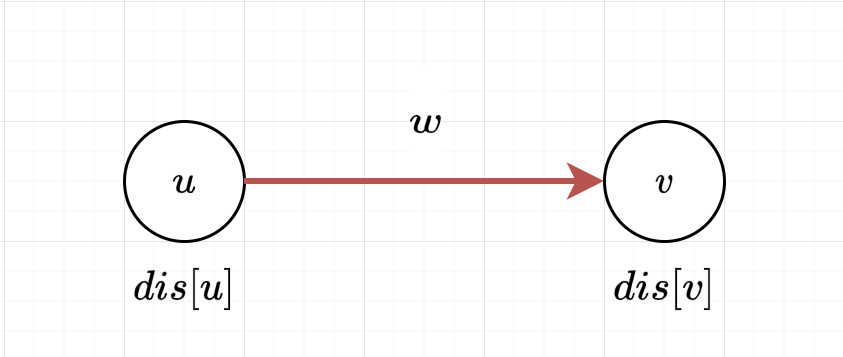
\includegraphics[scale=0.3]{images/relaxation.png}
        \end{center}
    \end{frame}
    
    \begin{frame}{SSSP - Dijkstra}
        \begin{itemize}
            \item 在剛剛講 BFS 時,因為圖的邊權都是 $1$,因此不會重複鬆弛
            \item 不過在邊權不一定是 $1$ 的圖上,如下圖
            \item 從 $1$ 開始,會先走到 $2, \ 3$,接著 $3$ 又被 $2$ 鬆弛
            \item 發現到 $3$ 會重複走到兩次
        \end{itemize}
        \vspace{2mm}
        \begin{center}
            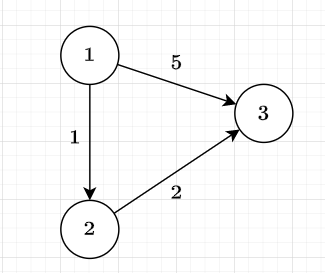
\includegraphics[scale=0.5]{images/example_dijkstra.png}
        \end{center}
    \end{frame}
    
    \begin{frame}{SSSP - Dijkstra}
        \begin{itemize}
            \item 重複鬆弛很顯然地會 TLE
            \item 那避免這個的方法就是從近的點開始先走
            \item 可以使用 priority\_queue 來解決
            \item priority\_queue 會幫我們把推進去的東西由小排到大!
        \end{itemize}
    \end{frame}
    
    \begin{frame}{SSSP - Dijkstra}
        \begin{columns}
            \begin{column}{0.5\textwidth}
                \begin{center}
                    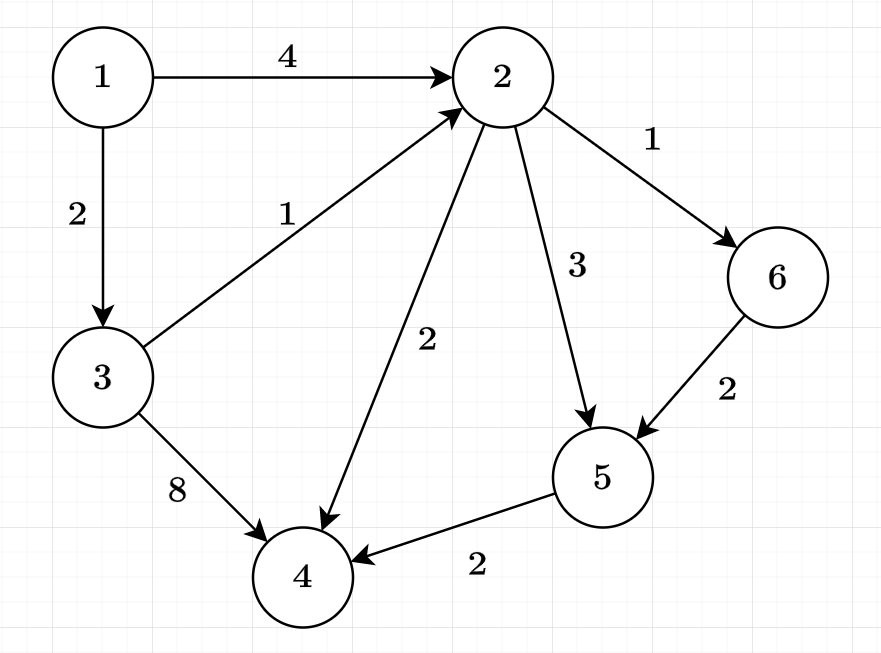
\includegraphics[scale=0.3]{images/dijkstra.png}
                \end{center}
            \end{column}
            \begin{column}{0.5\textwidth}
                (pq 按照起點走到 $u$ 的距離由小到大排序) 
                \begin{enumerate}
                    \item \texttt{push} $1$, $\texttt{dis[1] = 0}$, $\mathtt{pq} = \{3,2\}$
                    \item \texttt{pop} $3$ , $\texttt{dis[3] = 2}$, $\mathtt{pq} = \{2,4\}$
                    \item \texttt{pop} $2$ , $\texttt{dis[2] = 4}$, $\mathtt{pq} = \{6,4,5\}$
                    \item \texttt{pop} $6$ , $\texttt{dis[6] = 5}$, $\mathtt{pq} = \{4,5\}$
                    \item \texttt{pop} $4$ , $\texttt{dis[4] = 5}$, $\mathtt{pq} = \{5\}$
                    \item \texttt{pop} $5$ , $\texttt{dis[5] = 6}$
                \end{enumerate}
            \end{column}
        \end{columns}
    \end{frame}
    
    \begin{frame}{SSSP - Dijkstra}
        \begin{itemize}
            \item 一些實作細節 ><
            \item priority\_queue 裡面塞的是 pair,要按照距離排序,所以會是 $\{$距離,點$\}$
            \item 要避免從重複的點進行鬆弛,所以當點的最短距離 $<$ pq 中的距離,就 continue 
            \item 直接看 code 吧 ><
        \end{itemize}
    \end{frame}
    
    \begin{frame}{SSSP - Dijkstra CODE}
        \begin{center}
            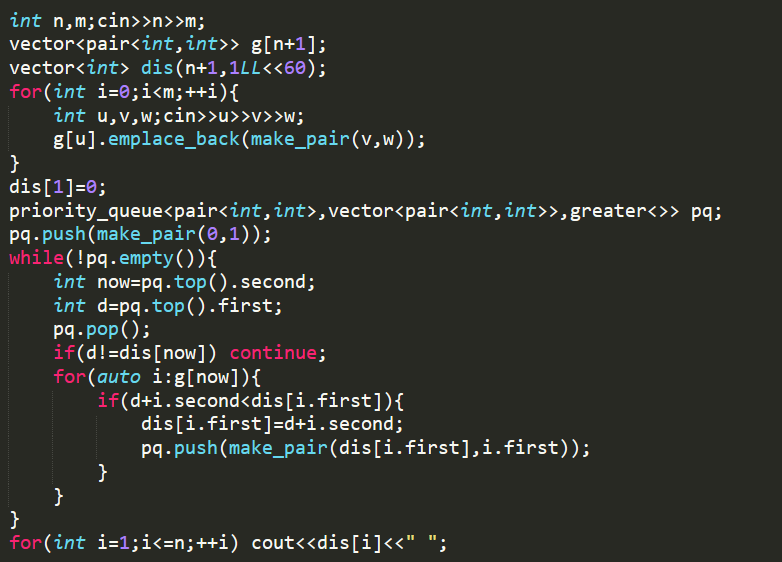
\includegraphics[scale=0.5]{code/dijkstra_code.png}
        \end{center}
    \end{frame}
    
    \begin{frame}{SSSP - Dijkstra}
        \begin{itemize}
            \item 每個邊最多會被 relax 到一次,所以更新 dis 的次數是 $|E|$
            \item 放進 pq 複雜度會是 $O(|E| \log |V|)$
            \item 將點的距離初始化的複雜度會是 $O(|V|)$
            \item 所以總時間複雜度會是 $O(|V| + |E| \log |V|)$
        \end{itemize}
    \end{frame}
    
    \begin{frame}{SSSP - 0-1 BFS}
        \begin{itemize}
            \item 觀察一下這張圖 owo
            \item 思考看看只有邊權 $0,1$ 的時候,Dijkstra 的 priority queue 會怎麼樣 
        \end{itemize}
        \begin{center}
            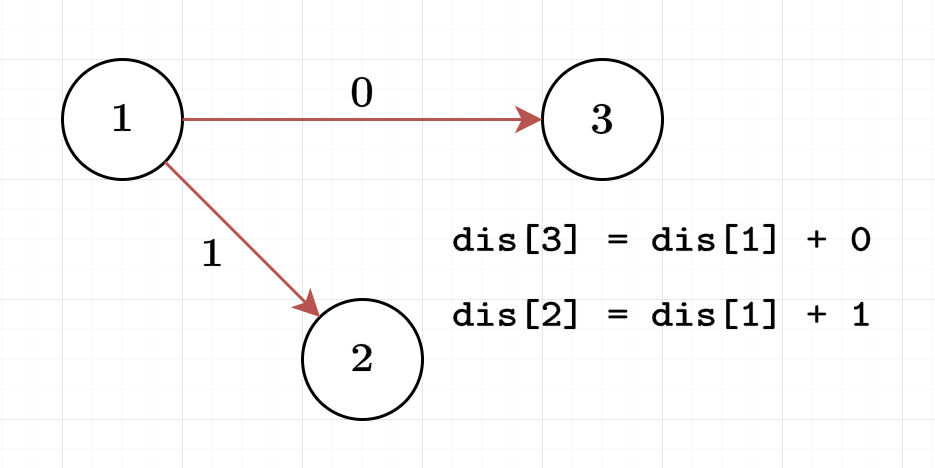
\includegraphics[scale=0.4]{images/01bfs.png}
        \end{center}
    \end{frame}
    
    \begin{frame}{SSSP - 0-1 BFS}
        \begin{itemize}
            \item 會發現當我們鬆弛了邊權是 $0$ 的邊 $u \rightarrow v$ 之後
            \item 走到 $v$ 的距離會跟走到 $u$ 的距離相同
            \item 所以在 priority queue 裡面會被排序到最前面!
            \item<2-> 只要用一個 deque,在邊權是 $0$ 的時候把點推到最前面
            \item<2-> 否則推到最後面就好了!
        \end{itemize}
    \end{frame}

    
    \begin{frame}{SSSP - 0-1 BFS}
        \begin{itemize}
            \item 如果使用 Dijkstra,複雜度會是 $O(|E| \log |V|)$
            \item 但只使用 deque 的話,複雜度就只要 $O(|V|+|E|)$ 
        \end{itemize}
    \end{frame}
    
    \begin{frame}{SSSP - 0-1 BFS Practice}
        \begin{block}{\href{https://www.codechef.com/problems/REVERSE}{CodeChef Chef and Reversing}}
        給一張有向圖,求最少需要翻轉幾條邊使得最少有一條路徑可以從$1$走到$N$
        \end{block}
        \begin{itemize}
            \item<2-> \sout{既然都放在0-1 BFS的例題了,那就想想它跟0/1有甚麼關係吧 XD}
            \item<3-> 要讓翻轉的邊數最少,那我們可以把它想成要經過最少條翻轉過的邊
            \item<4-> 再轉換一下,如果我們將原本的有向邊權重設為0,翻轉的邊權重設為1
            \item<5-> 那這不就是最短路徑問題了嗎!
            \item<6-> 當然,這題也是可以用 dijkstra 做的
        \end{itemize}
    \end{frame}
    
    \begin{frame}{如果今天的權重有負的怎麼辦?}
        \begin{itemize}
            \item Dijkstra 不能做負權嗎?
            \item<2-> 不能!因為如果有負權,路徑不一定會越走越長,鬆弛一次是不夠的!
            \item<3-> 介紹兩個可以處理負權的方法:Bellman-Ford, SPFA
        \end{itemize}
    \end{frame}
    %Bellman-Ford
    \begin{frame}{SSSP - Bellman-Ford}
        \begin{itemize}
            \item 鬆弛一次不夠,那就鬆弛很多次
            \item<2-> 其實就是暴力做
            \item<2-> 我們可以很輕易的證明:在沒有負環的圖上,起點$s$到所有點的最短路徑最多只會經過$|V|-1$條邊
            \item<2-> 所以跑$|V|-1$次,每次都對每個點鬆馳
            \item<3-> 時間複雜度:$O(|V|\times |E|)$
        \end{itemize}
    \end{frame}
    \begin{frame}{SSSP - Bellman-Ford Code}
        \begin{center}
             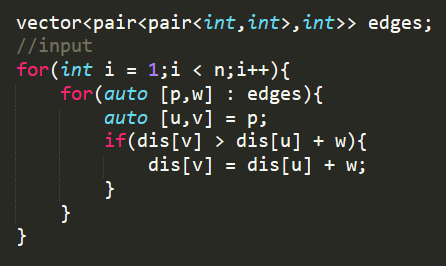
\includegraphics[scale=0.7]{code/BellmanFord_code.png}
        \end{center}
    \end{frame}
    \begin{frame}{SSSP - Bellman-Ford Practice}
        \begin{block}{\href{https://cses.fi/problemset/task/1673}{CSES High Score}}
        給一張有向圖,走過一條邊會得到 $w$ 分,邊權可正可負。問從 $1$ 走到 $n$ 最高可以拿到幾分,如果可以拿到無限大的分數,輸出 $-1$。
        \end{block}
        \begin{itemize}
            \item<2-> 把邊權乘以 $-1$ 之後,就變成最短路徑了
            \item<3-> 不過,這題可能會出現負環
            \item<4-> 要怎麼判斷 $1$ 走到 $n$ 會不會經過負環?
            \item<5-> 如果第 $|V|$ 次鬆弛到的點 $v$,可以從 $1 \rightarrow v \rightarrow n$ 的話
            \item<5-> 表示 $1$ 到 $n$ 會經過負環,可以使用兩次 DFS 來判斷
        \end{itemize}
    \end{frame}
    
    \begin{frame}{SSSP - Bellman-Ford}
        \begin{itemize}
            \item 已知在沒有負環的圖上,起點$s$到所有點的最短路徑最多只會經過$|V|-1$條邊
            \item<2-> 也就是說,在跑完$|V|-1$次後,我們已經找到起點到所有點的最短路
            \item<3-> 所以如果跑第$|V|$次時,還有節點被鬆弛,那就代表有負環
        \end{itemize}
    \end{frame}
    
    \begin{frame}[fragile]{SSSP - Bellman-Ford}
        \begin{lstlisting}[language=C++, basicstyle=\ttfamily\tiny]
fill(dis,dis+N,1e18);

dis[1] = 0;

for(int i = 0;i < n;i++){
    for(auto [u,v,w] : edges){
        if(dis[v] > dis[u] + w){
            dis[v] = dis[u] + w;
        }
    }
}

bool ok = false;
for(int i = 0;i < n;i++){
    for(auto [u,v,w] : edges){
        if(dis[v] > dis[u] + w){
            dis[v] = dis[u] + w;
            if(v==n) ok = true;
        }
    }
}
        \end{lstlisting}
    \end{frame}
    
    \begin{frame}{Frame Title}
        \begin{center}
             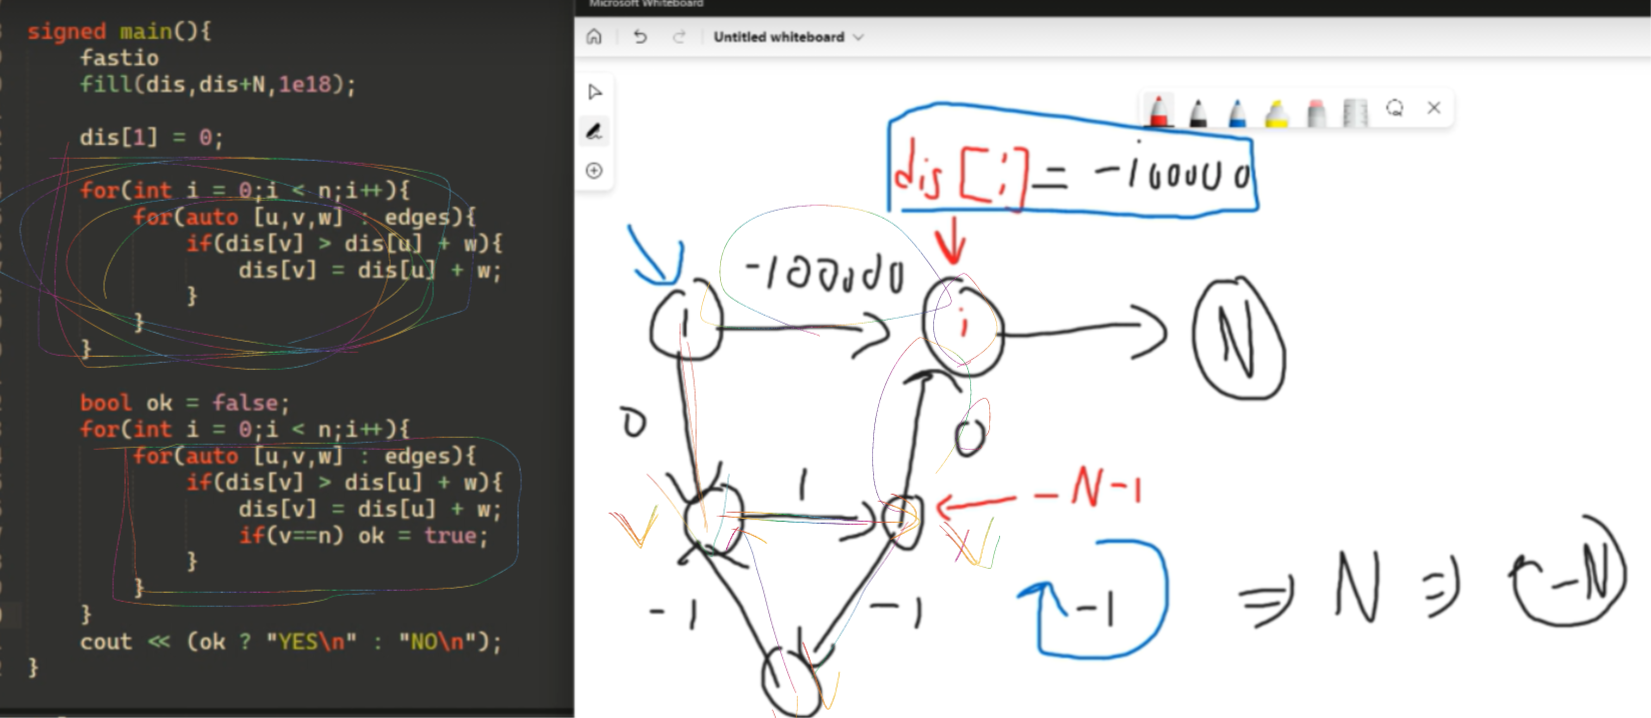
\includegraphics[scale=0.3]{images/image.png}
        \end{center}
    \end{frame}
    
    %spfa
    \begin{frame}{SSSP - SPFA}
        \begin{itemize}
            \item 全名叫 Shortest Path Faster Algorithm,它是 Bellman-Ford 的優化
            \item<2-> 實作上會把更新過的節點放進一個 queue,而且只檢查 queue 中節點連出去的邊
            \item<3-> 期望複雜度為$O(2|E|)$
            \item<4-> 但在最差的情況還是可能會跑到$O(|V|\times |E|)$
            \item<5-> 我們一樣可以用 SPFA 來檢查負環
            \item<5-> 如果有一個點被鬆弛了$|V|$次,那就代表有負環
        \end{itemize}
    \end{frame}
    
    \begin{frame}{SSSP - SPFA Code}
        \begin{center}
            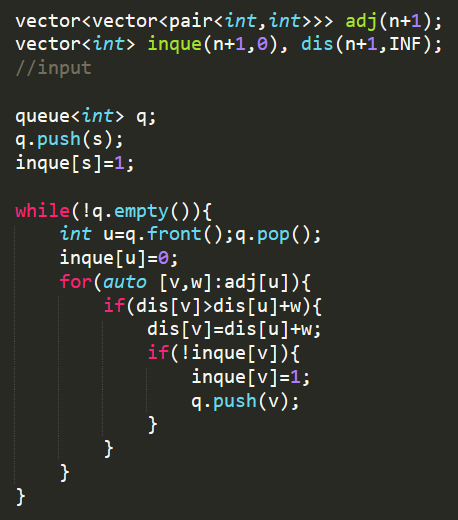
\includegraphics[scale=0.6]{code/SPFA_code.png}
        \end{center}
    \end{frame}
    
    \begin{frame}{APSP - 最直覺的作法}
        \begin{itemize}
            \item 既然已經學會了單點源的演算法
            \item 那要找全點對時,其實我們只要對所有的點都做一次 SSSP 就好了
            \item $|V|$ 次 Dijkstra: $O(|V||E| \log V)$,最糟會變成 $O(|V|^3 \log |V|)$
            \item $|V|$ 次 Bellman-Ford: $O(|V|(|V||E|))$,最糟會變成 $O(|V|^4)$
            \item 但其實有很好寫也更快速的方式,可以在 $O(|V|^3)$ 找完全點對!
        \end{itemize}
    \end{frame}
    
    %Floyd-Warshall
    \begin{frame}{APSP - Floyd-Warshall}
        \begin{itemize}
            \item 它其實就是 DP
            \item 我們可以令$dp[k][i][j]$表示從 $i$ 走到 $j$ 只經過 $[1,k]$ 的節點的最短距離
            \item 那這個的轉移式可以寫成\\ 
        \end{itemize}
        \vspace{3mm}
        $$dp[k+1][i][j]=\min\{dp[k][i][j],dp[k][i][k+1]+dp[k][k+1][j]\}$$
        \begin{itemize}
            \item<2-> 我們可以發現第一維可以滾掉
            \item<3-> 時間複雜度:$O(|V|^3)$
        \end{itemize}
    \end{frame}
    
    \begin{frame}{要注意的點}
        \begin{itemize}
            \item 初始化時,$dp[i][i]$ 要設成 $0$,其他初始化成 $\infty$
            \item 轉移的順序為 $k \rightarrow i \rightarrow j$
            \item 但在 \href{https://arxiv.org/pdf/1904.01210.pdf}{2019 年的一篇論文}中,提到不管哪個順序,只要跑三次都會是對的!
            \item 所以在使用時,如果真的忘記順序,跑三次就好了 XD
        \end{itemize}
    \end{frame}
    \begin{frame}{APSP - Floyd-Warshall Code}
        \begin{center}
            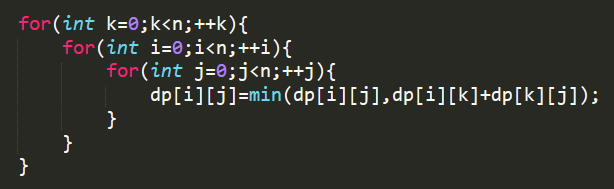
\includegraphics[scale=0.7]{code/FloydWarshall_code.png}
        \end{center}
    \end{frame}
    
    \section{樹論}
    \begin{frame}{樹的性質}
        \begin{columns}
            \begin{column}{0.65\textwidth}
                \begin{itemize}
                    \item 有 $|V|-1$ 條邊,兩兩節點之間有唯一的一條路徑
                    \item 增加一條邊後,必形成環
                    \item 去掉一條邊後,圖不再連通
                    \item 很多棵樹 $\Rightarrow$ 森林
                \end{itemize}
            \end{column}
            \begin{column}{0.35\textwidth}
                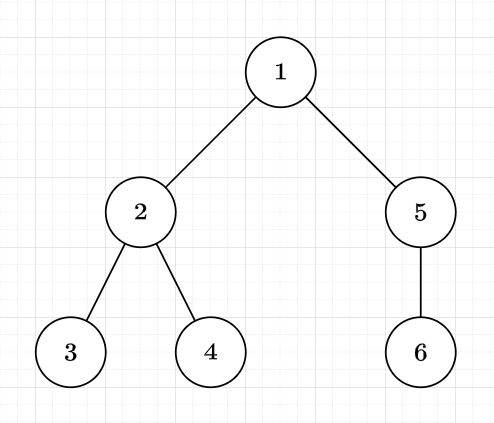
\includegraphics[width=\textwidth]{images/tree.png}
            \end{column}
        \end{columns}
    \end{frame}
    %樹直徑
    \section{樹直徑}
    \begin{frame}{熱身一下 ><}
        \begin{columns}
            \begin{column}{0.45\textwidth}
                \begin{itemize}
                    \item 找這棵樹上最長的路徑
                \end{itemize}
            \end{column}
            \begin{column}{0.5\textwidth}
                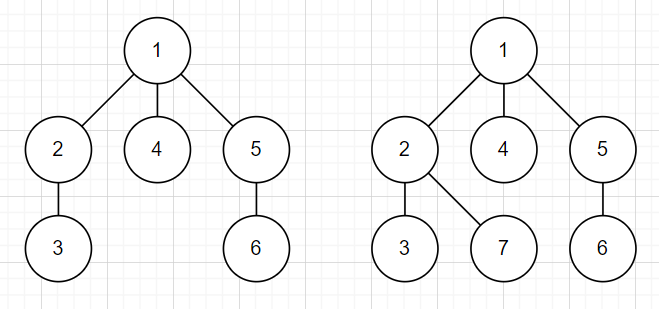
\includegraphics[width=\textwidth]{images/tree_ready.png}
            \end{column}
        \end{columns}
    \end{frame}
    \begin{frame}{甚麼是樹直徑?}
        \begin{columns}
            \begin{column}{0.45\textwidth}
            \begin{center}
                \begin{itemize}
                    \item 樹上最長的那條路徑
                    \item 可能會不只一條樹直徑
                \end{itemize}
            \end{center}
            \end{column}
            \begin{column}{0.5\textwidth}
                \begin{center}
                    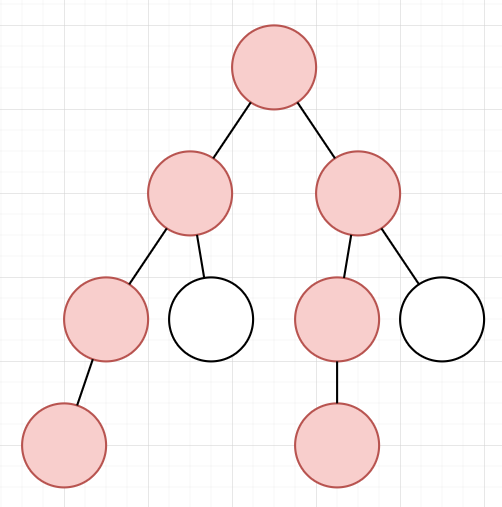
\includegraphics[scale=0.4]{images/tree_diameter.png}
                \end{center}
            \end{column}
        \end{columns}
        
    \end{frame}
    \begin{frame}{樹直徑實作}
        \begin{columns}
            \begin{column}{0.6\textwidth}
                \begin{itemize}
                    \item 如果權重沒有負的
                    \item 那我們可以找隨便一個點當起點,假設該點是 $s$
                    \item<2-> 先 dfs 找到距離點 $s$ 最遠的點 $u$
                    \item<3-> 再以 $u$ 為起點,dfs 找到距離 $u$ 最遠的點 $v$
                    \item<3-> $u$ 和 $v$ 之間的路徑,就是一條樹直徑
                    \item<4-> 為甚麼我們可以確定距離樹上任一點最遠的點,必定是樹直徑的兩端?
                    \item<5-> 等一下會證 owo
                \end{itemize}
            \end{column}
            \begin{column}{0.4\textwidth}
                \begin{center}
                    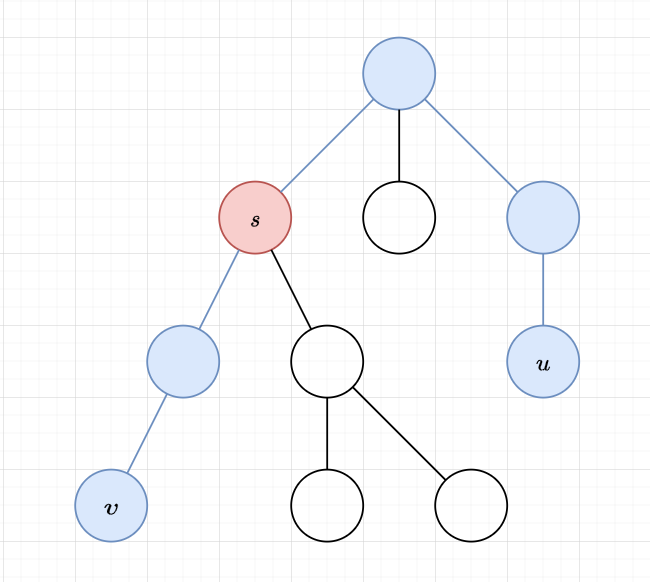
\includegraphics[scale=0.3]{images/tree_diameter_dfs.png}
                \end{center}
            \end{column}
        \end{columns}
    \end{frame}
    \begin{frame}{樹直徑實作}
        \begin{itemize}
            \item 那如果權重有負的怎麼辦?
            \item<2-> dp(後面樹 dp 會講)
        \end{itemize}
    \end{frame}
    \begin{frame}{兩次 dfs 作法的證明}
        \begin{itemize}
            \item 好欸 那我們回來證明「為甚麼做兩次 dfs 會是對的?」
        \end{itemize}
    \end{frame}
    \begin{frame}{兩次 dfs 作法的證明}
    \begin{columns}
    \begin{column}{0.5\textwidth}
        \begin{itemize}
            \item 現在假設$a$到$b$之間的路徑是樹直徑
            \item $dis(v,a)\geq dis(v,t)$ \\
            $\, \Longrightarrow (dis(v,a)-dis(v,c))\geq (dis(v,t)-dis(v,c))$\\
            $\, \Longrightarrow dis(a,c)\geq dis(c,t)$ 
            \item<2-> 將位在樹直徑上左半邊的節點當作根
            \item<2-> 那它的子樹深度不會超過該節點到樹直徑最左端的距離。
            \item<3-> 同理,我們也可以推出右半邊也是如此
            \item<4-> 所以這邊的結論是:樹直徑上任一節點$x$,其子樹深度都不會超過$\min(dis(x,a),dis(x,b))$
        \end{itemize}
    \end{column}
    \begin{column}{0.5\textwidth}
        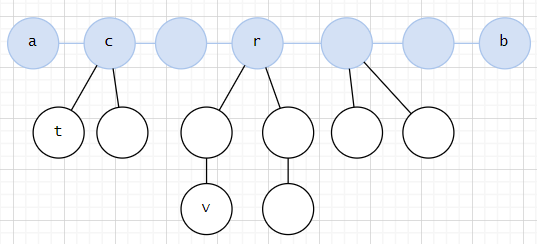
\includegraphics[width=\textwidth]{images/dfs_proof.png}
    \end{column}
    \end{columns}
    \end{frame}
    \begin{frame}{兩次 dfs 作法的證明}
        \begin{itemize}
            \item 我們現在需要證明的是:為甚麼第一次 dfs 找到的點會是樹直徑的其中一端?
            \item Claim: 對於所有點$i$,找到距離它最遠的點$j$,則$j$必定滿足$j=a$ or $j=b$ 
        \end{itemize}
    \end{frame}
    \begin{frame}{兩次 dfs 作法的證明}
    \begin{columns}
    \begin{column}{0.5\textwidth}
        \begin{itemize}
            \item 我們可以用剛剛證明出來的結論得出
            \item<2-> \texttt{if} $j=j_1,$\\
            $\,dis(i,j_1)=dis(i,r)+dis(r,j_1)\leq dis(i,r)+dis(r,a)=dis(i,a)$
            \item<2-> \texttt{if} $j=j_2,$\\
            $\,dis(i,j_2)= dis(i,r)+dis(r,j_2)\leq dis(i,r)+dis(r,a)=dis(i,a)$
        \end{itemize}
    \end{column}
    \begin{column}{0.5\textwidth}
        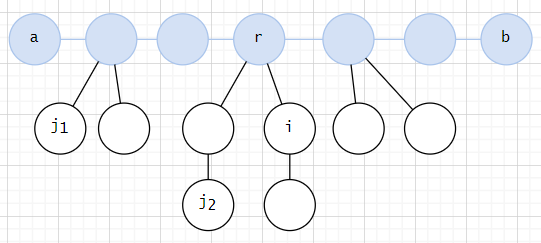
\includegraphics[width=\textwidth]{images/dfs_proof_2.png}
    \end{column}
    \end{columns}
    \end{frame}
    \begin{frame}
        \frametitle{兩次 dfs 作法的證明}
        \begin{itemize}
            \item 參考資料 \href{https://codeforces.com/blog/entry/101271}{Diameter of a tree and its applications}
        \end{itemize}
    \end{frame}
    \begin{frame}{這是一題很裸很裸的題目 ><}
        \begin{block}{\href{https://cses.fi/problemset/task/1131}{CSES Tree Diameter}}
        找樹直徑長度
        \end{block}
    \end{frame}
    
    \begin{frame}
        \frametitle{樹圓心}
        \begin{itemize}
            \item 樹圓心:樹直徑中間的那個點 (不一定會跟重心一樣)
            \item 樹圓心可能會有兩個
            \item 以樹圓心為根時,樹的深度會最小
        \end{itemize}
        \begin{center}
            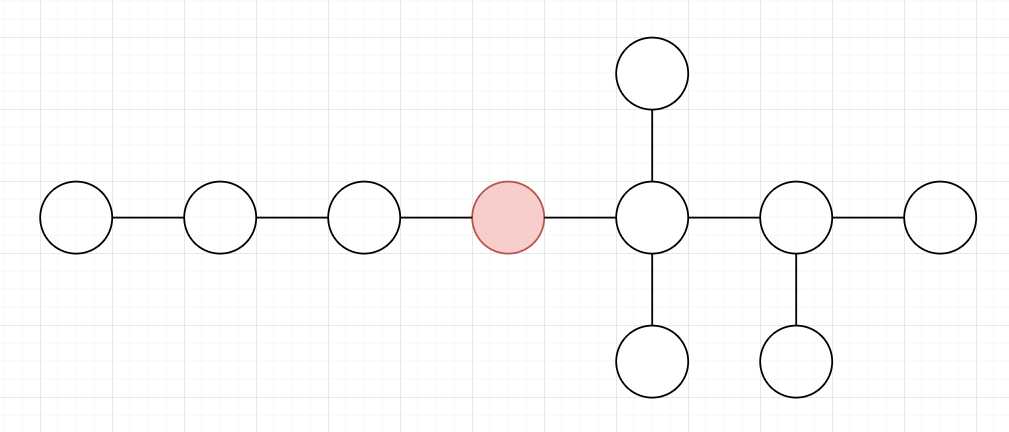
\includegraphics[scale=0.25]{images/tree_center.png}
        \end{center}
    \end{frame}
    
    \begin{frame}
        \frametitle{直徑的性質}
        \begin{itemize}
            \item 把樹上樹直徑的邊拔掉,會得到森林
            \item 每棵樹的節點會以在直徑上的點為根
            \item 若以點 $u$ 為根的樹,它的深度不會超過到直徑端點 $a$ 的距離 $dis(u,a)$
        \end{itemize}
        
        \begin{center}
            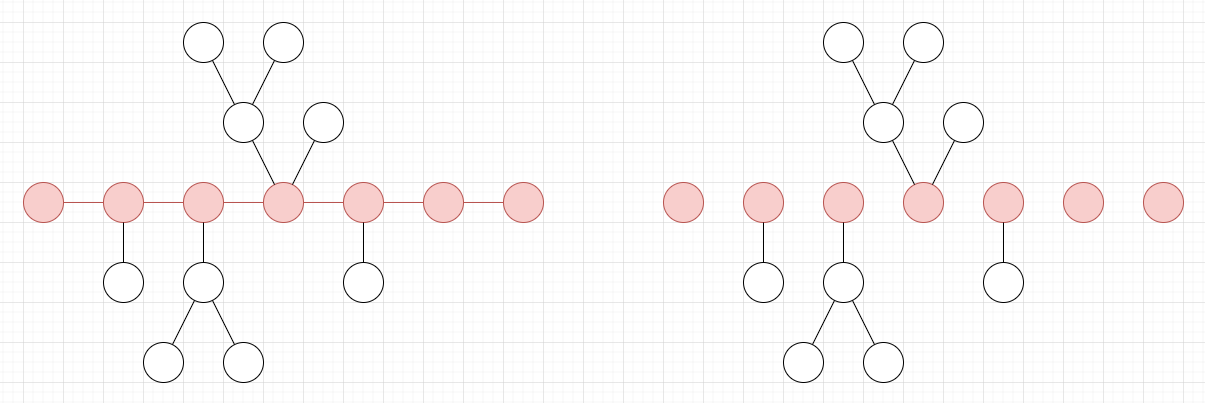
\includegraphics[scale=0.4]{images/tree_diameter_property.png}
        \end{center}
    \end{frame}
    
    %樹重心
    \section{樹重心}
    \begin{frame}{甚麼是樹重心?}
        \begin{itemize}
            \item 拔除後可以使所有連通塊的最大值最小的點
            \item 把它拔掉以後,每個連通塊大小都不超過 $N/2$ 
            \item 樹重心可能不只一個,但最多就兩個
            \item 最常見的應用是重心剖分 (Centroid Decomposition),但我們不會講
        \end{itemize}
    \end{frame}
    \begin{frame}{甚麼是樹重心?}
        \begin{center}
            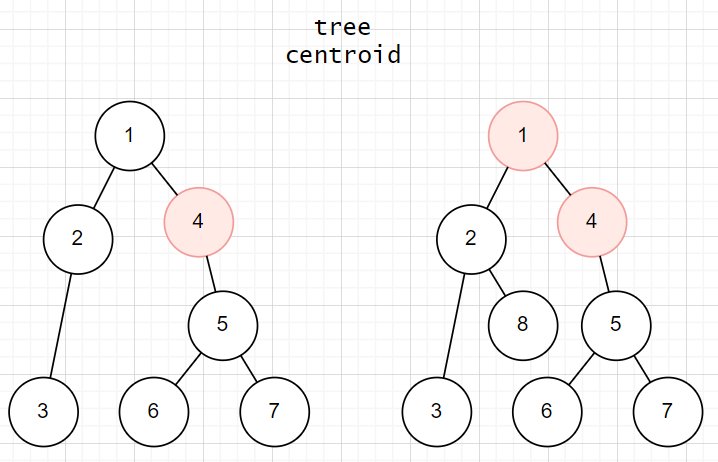
\includegraphics[scale=0.7]{images/tree_centroid.png}
        \end{center}
    \end{frame}
    \begin{frame}{樹重心實作}
        \begin{itemize}
            \item 隨便找一個節點,把它當根
            \item DFS 去找每個點的子樹大小
            \item<2-> 把該點拔去以後,會產生兩種連通塊
            \item<2-> 分別是「孩子的子樹大小」和「節點數 - 自己的子樹大小」
            \item<3-> 根據前面的定義,如果大小都不超過 $N/2$,那它就是樹重心(之一)
        \end{itemize}
    \end{frame}
    \begin{frame}{這是一題很裸很裸的題目 ><}
        \begin{block}{\href{https://neoj.sprout.tw/problem/293/}{NEOJ 293 樹重心}}
        給一棵樹,找樹重心,若有多個,那就輸出編號最小的
        \end{block}
    \end{frame}
    
    %Euler Tour
    \section{樹壓平 (Euler Tour)}
    \begin{frame}
        \frametitle{樹壓平}
        \begin{itemize}
            \item 現在給你一棵樹,能不能用一個序列表示這棵樹?
            \item<2-> 把 DFS 的順序紀錄下來 owo
        \end{itemize}
    \end{frame}
    
    \begin{frame}
        \frametitle{樹壓平}
        \begin{columns}
            \begin{column}{0.6 \textwidth}
                \begin{itemize}
                    \item 對每個點,紀錄進入這個點和離開這個點的時間
                    \item 我們會得到一個長度是 $2n$ 的序列
                    \item<2-> 在 $in[u]$ 和 $out[u]$ 之間的點都是 $u$ 的子孫
                    \item<3-> 可以搭配資料結構維護子樹
                    \item<4-> 因為是把樹壓成序列,被稱作「樹壓平」
                \end{itemize}
            \end{column}
            \begin{column}{0.4 \textwidth}
                \begin{center}
                    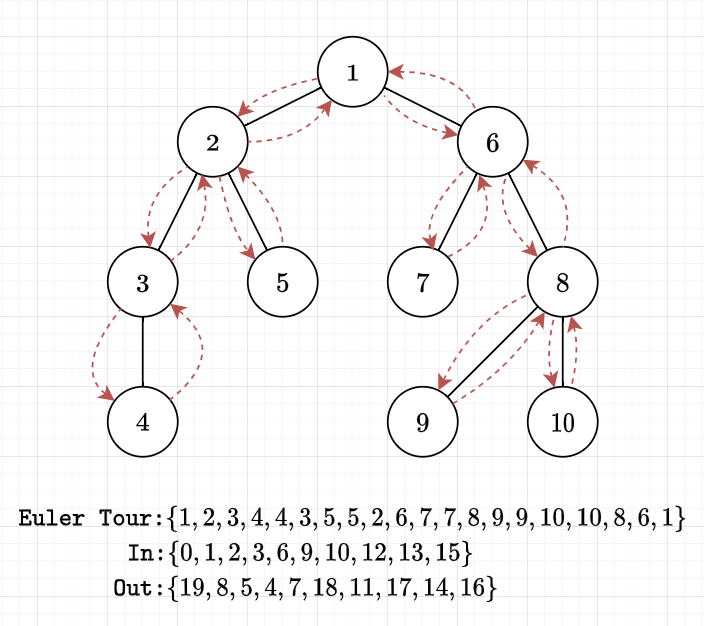
\includegraphics[scale=0.3]{images/euler_tour.png}
                \end{center}
            \end{column}
        \end{columns}
    \end{frame}
    
    %dp
    \section{樹 dp}
    \begin{frame}{樹 dp}
        \begin{itemize}
            \item 就是在樹上做 dp
            \item 通常節點的狀態與子樹有關,從孩子轉移過來
            \item 我們可以先來看一個簡單的例子
        \end{itemize}
    \end{frame}
    
    \begin{frame}{這是一個很簡單的例子 ><}
        \begin{block}{\href{https://cses.fi/problemset/task/1674/}{CSES Subordinates}}
        給一棵樹,問每個節點的子樹大小(不包含自己)\\
        $1\leq n \leq 2 \cdot 10^5$
        \end{block}
        \begin{columns}
            \begin{column}{0.8\textwidth}
                \begin{itemize}
                    \item 以範測為例,我們可以畫出右圖
                    \item<2-> 若這題用暴力解決,顯然會 TLE,我們可以考慮一下 dp 的作法
                    \item<3-> 令$dp[i]=$節點$i$的子樹大小
                    \item<4-> 令$j$為節點$i$的子節點,令$cnt$為$i$的子節點個數
                    \item<5-> 那你會發現$dp[i]= \sum dp[j]+cnt$
                    \item<5-> 遞迴的時候處理
                \end{itemize}
            \end{column}
            \begin{column}{0.25\textwidth}
                \begin{center}
                    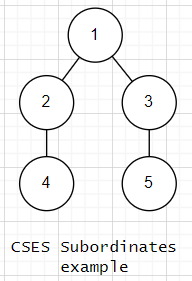
\includegraphics[scale=0.8]{images/CSES_Subordinates_example.png}
                \end{center}
            \end{column}
        \end{columns}
    \end{frame}
    
    % 記得補 DP 作法
    \begin{frame}{樹直徑}
        \begin{block}{\href{https://cses.fi/problemset/task/1131/}{CSES Tree Diameter}}
        找樹直徑長度\\
        $1\leq n \leq 2 \cdot 10^5$
        \end{block}
        \begin{itemize}
            \item<2-> 剛剛講過兩次 DFS 的作法了 ><
            \item<2-> 可是在有負權的時候,不能直接 DFS QwQ
            \item<2-> 所以我們要用樹 DP
        \end{itemize}
    \end{frame}
    
    \begin{frame}{樹直徑}
        \begin{block}{\href{https://cses.fi/problemset/task/1131/}{CSES Tree Diameter}}
        找樹直徑長度\\
        $1\leq n \leq 2 \cdot 10^5$
        \end{block}
        \begin{itemize}
            \item 設 $dp_1[u]$ 表示 $u$ 往下走的\textbf{最長}路徑
            \item 設 $dp_2[u]$ 表示 $u$ 往下走的\textbf{次長}路徑
            \item 那樹直徑就會是所有的 $dp_1[u] + dp_2[u]$ 中的最大值 owo
        \end{itemize}
    \end{frame}
    
    \begin{frame}{Practice}
        \begin{block}{\href{https://codeforces.com/problemset/problem/1528/A}{Codeforces 1528A Parsa's Humongous Tree}}
        給你一棵樹,每個節點 $u$ 上有兩個權值 $l_u, r_u$,你可以對每個節點寫上一個數字 $a_u$。你希望可以知道最大的 $\sum_{(u,v)\in E} |a_u-a_v|$ 是多少?
        \end{block}
        \begin{itemize}
            \item<2-> 這題應該可以很顯然地發現只需要注意$l$和$r$
            \item<3-> 可以開 $dp[u][0]$ 表示 $a_u = l_u$ 時子樹的最大價值
            \item<3-> 同理,開 $dp[u][1]$ 表示 $a_u = r_u$ 時子樹的最大價值
            \item<4-> 然後這樣就結束了
        \end{itemize}
    \end{frame}
    
    \begin{frame}{Practice}
        \begin{block}{\href{https://codeforces.com/problemset/problem/1646/D}{Codeforces 1646D Weight the Tree}}
        給你一棵樹,你要將所有的點標上一個權值。定義好的節點表示它的權值等於與其相鄰的節點的權值總和。請找到可以讓好的節點最多,且總權值和最小的一種方法。
        \end{block}
        \begin{itemize}
            \item<2-> 觀察到當 $n \ge 3$ 的時候,好的節點一定不會與好的節點相鄰
            \item<3-> 定義 DP 式 $dp[u][0]$ 表示整個子樹的最優解,且 $u$ 是壞的節點
            \item<3-> 同理,定義 $dp[u][1]$ 表示整個子樹的最優解,且 $u$ 是好的節點
            \item<4-> 在轉移時,好的節點只能從壞的節點轉移
            \item<5-> 由於要輸出一種方案,在轉移時,順便維護轉移來的人即可
        \end{itemize}
    \end{frame}
    
    
    \section{換根 DP (Rerooting DP)}
    \begin{frame}{換根 dp (Rerooting DP)}
        \begin{itemize}
            \item 有時候題目會希望你找到對於所有點當根的 DP 答案
            \item 假設一次樹 DP 要花 $O(n)$,每一次都從某個點開始 DFS 就要 $O(n^2)$ 了耶 owo
            \item 所以我們不能夠直接做 $n$ 次
        \end{itemize}
    \end{frame}
    
    
    \begin{frame}{換根 dp (Rerooting DP)}
        \begin{columns}
            \begin{column}{0.6 \textwidth}
                \begin{itemize}
                    \item 在這裡我們要用到換根的想法
                    \item 假設我們知道節點 $u$ 的 DP 值
                    \item 想要知道與 $u$ 相鄰的點 $v$ 當根的 DP 值
                    \item 我們可以在 $O(1)$ 或 $O(\log n)$ 的時間做完
                    \item 這個技巧在日本叫做「全方位木 DP」
                \end{itemize}
            \end{column}
            \begin{column}{0.4 \textwidth}
                \begin{center}
                    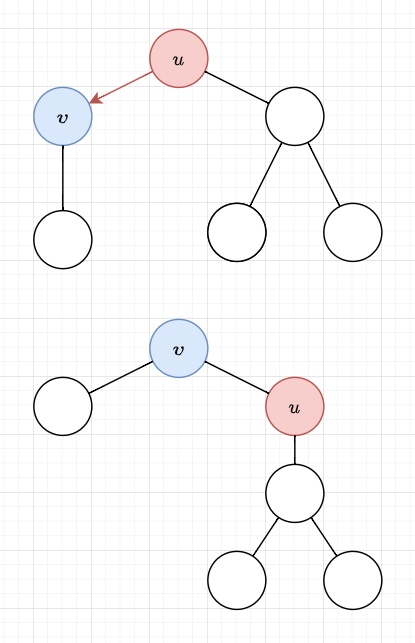
\includegraphics[scale=0.35]{images/reroot.png}
                \end{center}
            \end{column}
        \end{columns}
    \end{frame}
    
    \begin{frame}{換根 dp (Rerooting DP)}
        \begin{columns}
            \begin{column}{0.6 \textwidth}
                \begin{itemize}
                    \item 會換根之後,要怎麼換才能得到所有點的值?
                    \item<2-> 什麼順序可以讓我們剛好走過樹上每個點?
                    \item<3-> Euler Tour!
                    \item<4-> 一共只會做 $O(n)$ 次換根
                    \item<4-> 複雜度比起每次重新做好很多!
                    \item<5-> 直接看例題應該比較好懂 owo
                \end{itemize}
            \end{column}
            \begin{column}{0.4 \textwidth}
                \begin{center}
                    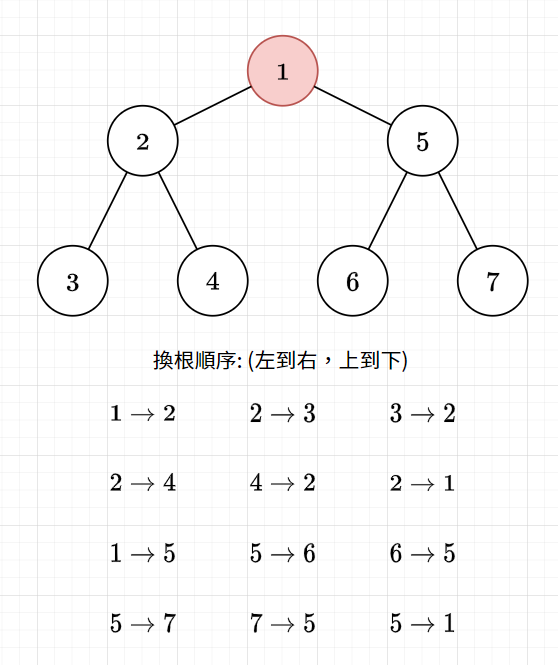
\includegraphics[scale=0.35]{images/reroot_order.png}
                \end{center}
            \end{column}
        \end{columns}
    \end{frame}
    
    \begin{frame}{換根 DP Practice}
        \begin{block}{\href{https://codeforces.com/contest/1092/problem/F}{Codeforces 1092F Tree with Maximum Cost}}
        給你一棵樹,每個點 $i$ 都有一個點權 $a_i$,定義以某個點 $v$ 為根時,樹的價值為 $\sum_{i=1}^n dist(v,i) \cdot a_i$。問這棵樹的最大價值可以是多少? \\
        \vspace{5mm}
        $1 \le n \le 2 \cdot 10^5$
        \end{block}
        \begin{itemize}
            \item<2-> 首先,如果我們固定了一個點(例如:$1$)當根
            \item<2-> 要怎麼計算這棵樹的價值呢?
        \end{itemize}
    \end{frame}
    
    \begin{frame}{換根 DP Practice}
        \begin{block}{\href{https://codeforces.com/contest/1092/problem/F}{Codeforces 1092F Tree with Maximum Cost}}
        給你一棵樹,每個點 $i$ 都有一個點權 $a_i$,定義以某個點 $v$ 為根時,樹的價值為 $\sum_{i=1}^n dist(v,i) \cdot a_i$。問這棵樹的最大價值可以是多少? \\
        \vspace{5mm}
        $1 \le n \le 2 \cdot 10^5$
        \end{block}
        \begin{columns}
            \begin{column}{0.6\textwidth}
                \begin{itemize}
                    \item 觀察到 $dist(v,i)$ 其實就是 $i$ 的深度
                    \item 因此我們設 $dp[v]$ 表示 $v$ 的子樹的總價值
                    \item 轉移式: $dp[v] = \sum_{u \in v_c} dp[u] + \texttt{dep}[v] \cdot a_i$
                    \item<2-> 找到以 $1$ 為根的答案了,然後呢 ><
                \end{itemize}
            \end{column}
            \begin{column}{0.4\textwidth}
                \begin{center}
                    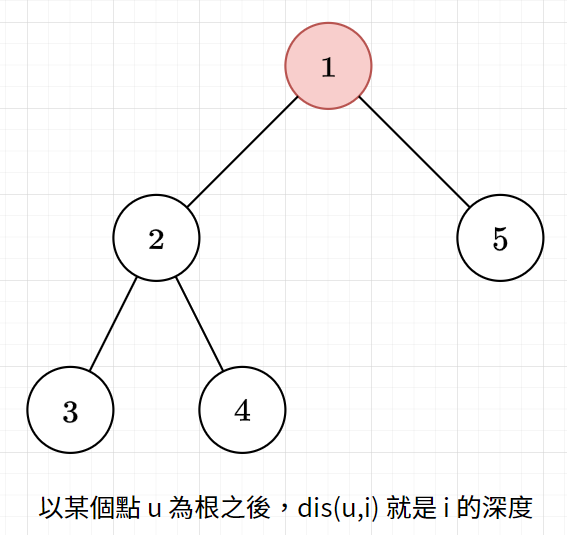
\includegraphics[scale=0.25]{images/cf1072f.png}
                \end{center}
            \end{column}
        \end{columns}
    \end{frame}
    
    \begin{frame}{換根 DP Practice}
        \begin{columns}
            \begin{column}{0.6\textwidth}
                \begin{itemize}
                    \item 再來我們要想如何換根 owo
                    \item<2-> 根從 $u \rightarrow v$ 最直接的改變就是深度
                    \item<2-> $v$ 的子樹深度都會少 $1$,$u$ 的子樹深度都會多 $1$
                    \item<3-> $dp[u]$ 不會再包含 $v$ 的子樹,$dp[u]$ 要減少 $dp[v]$
                    \item<4-> $u$ 子孫深度都多 $1$,$dp[u]$ 要增加 $\sum_{i \in U} a_i$ 
                    \item<4-> $v$ 子孫深度都少 $1$,$dp[v]$ 要減少 $\sum_{j \in V} a_j$
                    \item<5-> $dp[v]$ 要加上 $dp[u]$,因為 $u$ 變成 $v$ 的孩子了
                    \item<6-> 實作上會再開一個 $sum[u]$ 表示 $\sum_{i \in U} a_i$ 
                \end{itemize}
            \end{column}
            \begin{column}{0.4\textwidth}
                \begin{center}
                    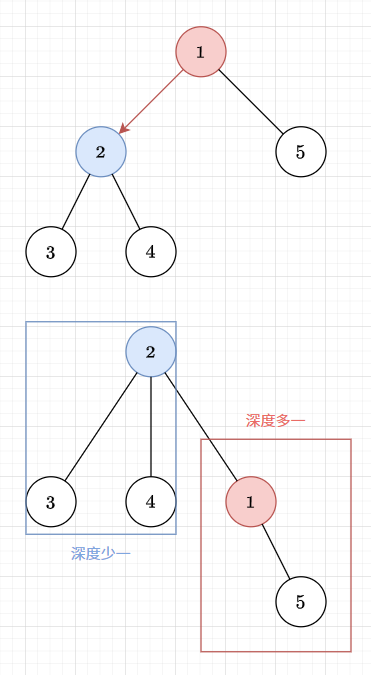
\includegraphics[scale=0.36]{images/cf1072f_2.png}
                \end{center}
            \end{column}
        \end{columns}
    \end{frame}
    
    \begin{frame}{換根 DP Practice}
        \begin{block}{\href{https://codeforces.com/contest/1092/problem/F}{Codeforces 1092F Tree with Maximum Cost}}
        給你一棵樹,每個點 $i$ 都有一個點權 $a_i$,定義以某個點 $v$ 為根時,樹的價值為 $\sum_{i=1}^n dist(v,i) \cdot a_i$。問這棵樹的最大價值可以是多少? \\
        \vspace{5mm}
        $1 \le n \le 2 \cdot 10^5$
        \end{block}
        \begin{itemize}
            \item 所以我們花了 $O(n)$ 的時間找到某個點為根的答案
            \item 接著一次換根需要 $O(1)$,我們換了 $O(n)$ 次
            \item 複雜度是 $O(n)$,比起做 $n$ 次 DFS 快了超級多 owo
        \end{itemize}
    \end{frame}
    
    %DSU
    \section{並查集}
    \begin{frame}{甚麼是並查集?}
        \begin{itemize}
            \item 並查集,又叫 DSU(Disjoint Set Union)
            \item 一種資料結構,可以維護一些集合,支援\textbf{合併}和\textbf{查詢}兩種操作
        \end{itemize}
        \begin{center}
            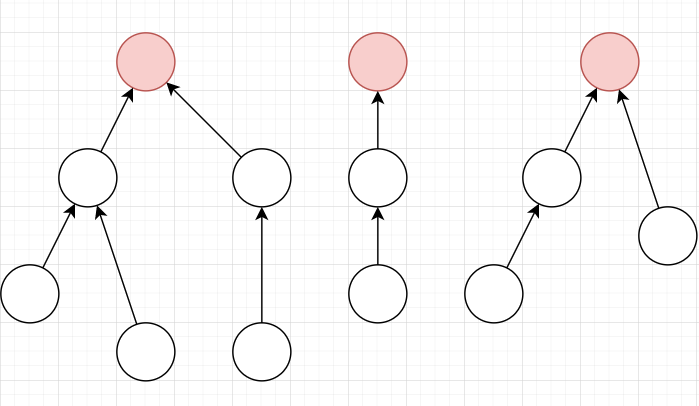
\includegraphics[scale=0.5]{images/dsu.png}
        \end{center}
    \end{frame}
    \begin{frame}{操作}
        \begin{itemize}
            \item 每個集合都是一棵樹
            \item<2-> 最初每個點都是一個集合,且自己就是自己的根節點的父節點
            \item<3-> 要查詢兩個點是否位於同一個集合,就看他們的祖先是不是同一個
            \item<4-> 要把兩個集合合併,就讓一個集合的根節點的父節點變成另一個集合的根節點
        \end{itemize}
    \end{frame}
    \begin{frame}{code}
        \begin{center}
            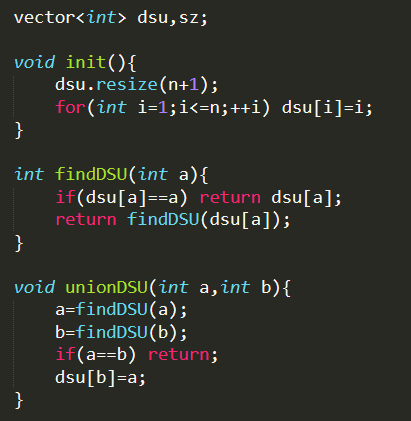
\includegraphics[scale=0.6]{code/dsu_basic.png}
        \end{center}
    \end{frame}
    \begin{frame}{優化}
        \begin{itemize}
            \item 你會發現合併以後可能會有很長的鍊
            \item<2-> 如果是一條鍊,那麼每次向上找祖先時,複雜度最差會是 $O(n)$
            \item<3-> 所以我們的目標是:\\
            不讓他找祖先時需要走那麼多步,又或者是說,乾脆不要讓他有機會形成一條鏈
        \end{itemize}
    \end{frame}
    \begin{frame}{優化 - 路徑壓縮}
        \begin{columns}
            \begin{column}{0.6\textwidth}
                \begin{itemize}
                    \item 就是把路變短
                    \item<2-> 讓每個點往上走一步就會到根節點
                    \item<2-> 在遞迴(findDSU)的時候做掉一整條
                    \item<2-> 這樣複雜度會變 $O(\log n)$
                \end{itemize}
            \end{column}
            \begin{column}{0.4\textwidth}
                \begin{center}
                     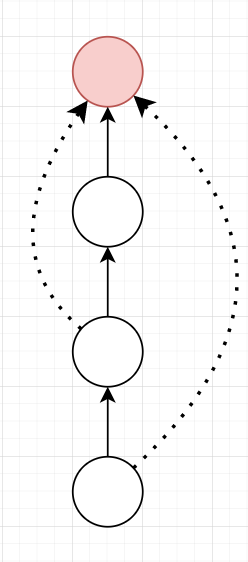
\includegraphics[scale=0.35]{images/path_compression.png}
                \end{center}
            \end{column}
        \end{columns}
    \end{frame}
    \begin{frame}{code}
        \begin{center}
            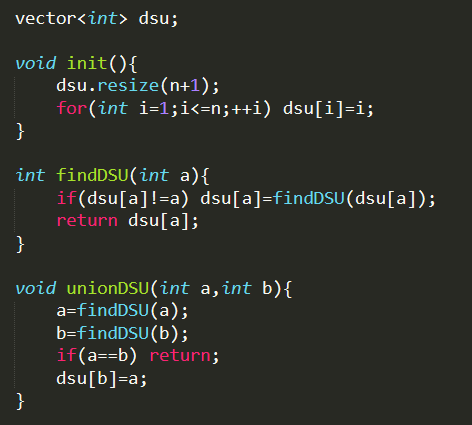
\includegraphics[scale=0.6]{code/dsu_compression.png}
        \end{center}
    \end{frame}
    \begin{frame}{優化 - 啟發式合併}
        \begin{itemize}
            \item 除了把路變短,我們可以一開始就讓路不要那麼長
            \item<2-> 在合併的時候將較大集合的根節點當作小集合的根節點的父節點
            \item<3-> 這樣每往上走一個點,子樹大小至少會變兩倍
            \item<4-> 因此樹的深度最多會是 $O(\log n)$
            \item<4-> 換句話說,最多走 $O(\log n)$ 步就會抵達根節點
            \item<5-> 實作的話多維護一個集合大小就好
        \end{itemize}
    \end{frame}
    \begin{frame}{優化 - 啟發式合併}
        \begin{center}
            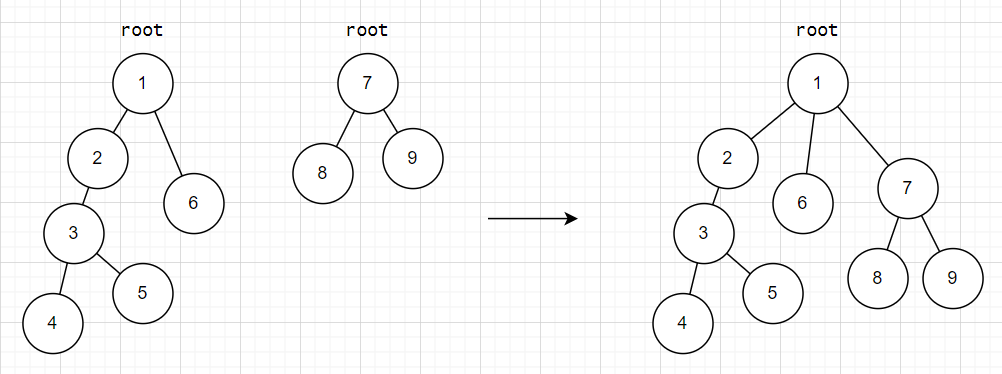
\includegraphics[scale=0.7]{images/DSU_merge.png}
        \end{center}
    \end{frame}
    \begin{frame}{code}
        \begin{center}
            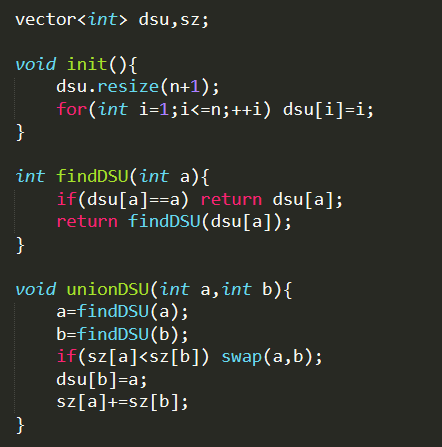
\includegraphics[scale=0.6]{code/dsu_merge.png}
        \end{center}
    \end{frame}
    \begin{frame}{優化}
        \begin{itemize}
            \item 好耶好快
            \item 還可以更快!!!
            \item<2-> 兩個優化一起用!
            \item<3-> 兩個一起用的時候複雜度是 $O(\alpha(n))$
            \item<3-> $\alpha$ 是一個成長率超級無敵霹靂小的函數
            \item<3-> 非常接近常數
        \end{itemize}
    \end{frame}
    \begin{frame}{code}
        \begin{center}
            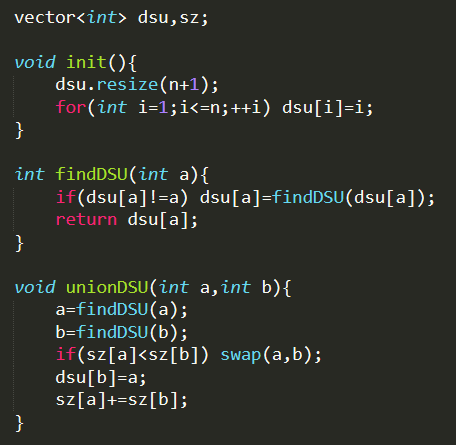
\includegraphics[scale=0.6]{code/dsu_c_m.png}
        \end{center}
    \end{frame}
    \begin{frame}{優化}
        \begin{itemize}
            \item 但並不是所有題目都可以用以上兩種優化
            \item 因為這兩種優化會改到樹本身的結構
        \end{itemize}
    \end{frame}
    \begin{frame}{喵喵喵喵喵}
        \begin{center}
            現在來看一些可以寫的例題 ><
        \end{center}
    \end{frame}
    \begin{frame}{Practice}
        \begin{block}{\href{https://codeforces.com/problemset/problem/1594/D}{CodeForces D. The Number of Imposters}}
        imposter 只會說謊,crewmate 只會說真話\\
        給$m$個線索,例如:$a$說$b$是 crewmate\\
        在符合這些關係的前提下,輸出最多會有幾個 imposter,若他給的線索已經造成矛盾,那就輸出 -1。
        \end{block}
        \begin{itemize}
            \item<2-> 轉換一下題目
            \item<2-> 當 $a$ 說 $b$ 是 crewmate,$a$ 和 $b$ 的身分相同
            \item<2-> 當 $a$ 說 $b$ 是 imposter,$a$ 和 $b$ 的身分相反
            \item<3-> 只考慮第二種邊,題目就變成
            \item<3-> 給你一張圖,然後判斷它是不是二分圖
            \item<4-> 就 DFS 塗顏色就好了 R
            \item<5-> 對!這題就這樣
            \item<6-> 那我們來看一下另一題
        \end{itemize}
    \end{frame}
    \begin{frame}{Practice}
         \begin{block}{\href{https://codeforces.com/edu/course/2/lesson/7/2/practice/contest/289391/problem/J}{CodeForces DSU edu step2 J First Non-Bipartite Edge}}
         一開始圖上只有$n$個點,接著每次加入一條邊\\請找出一條邊,使得二分圖加上該邊後不是二分圖
        \end{block}
        \begin{itemize}
            \item<2-> 這題其實有二分搜 + DFS 塗色的做法
            \item<2-> 可是我們要用 DSU owo
        \end{itemize}
    \end{frame}

    \begin{frame}
        \frametitle{DSU 判二分圖}
        \begin{columns}
            \begin{column}{0.6 \textwidth}
                \begin{itemize}
                    \item 思考一下 DFS 判斷二分圖的方式
                    \item 我們會先決定好起點的顏色
                    \item 接著從 $u$ 走到 $v$ 時,將 $v$ 和 $u$ 塗上不同的顏色
                \end{itemize}
            \end{column}
            \begin{column}{0.4 \textwidth}
                \begin{center}
                    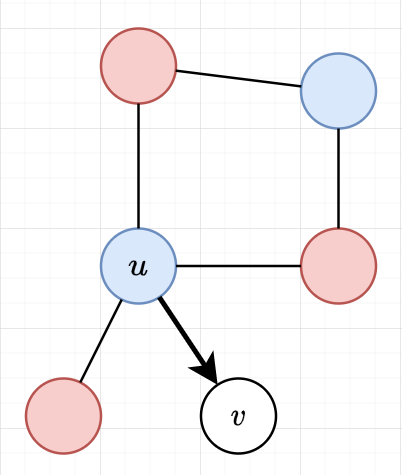
\includegraphics[scale=0.4]{images/bipartite.png}
                \end{center}
            \end{column}
        \end{columns}
    \end{frame}
    
    \begin{frame}
        \frametitle{DSU 判二分圖}
        \begin{columns}
            \begin{column}{0.6 \textwidth}
                \begin{itemize}
                    \item 既然我們會去決定 $u$ 的顏色再進行塗色
                    \item 那如果我們把兩種塗色方法一起做呢?
                    \item 對每個點都開兩個不同的點,並分別標上 $1$ 和 $0$
                    \item 在塗色的時候,把 $u$ 連 $v'$,$v$ 連 $u'$
                    \item 最後會建出兩個塗上不同顏色的二分圖
                \end{itemize}
            \end{column}
            \begin{column}{0.4 \textwidth}
                \begin{center}
                    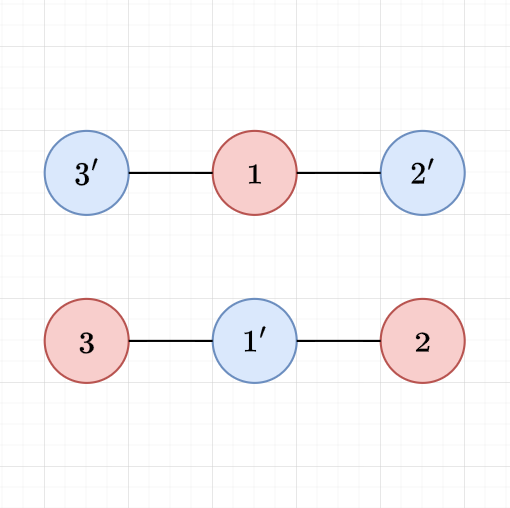
\includegraphics[scale=0.3]{images/bipartite_dsu.png}
                \end{center}
            \end{column}
        \end{columns}
    \end{frame}
    
    \begin{frame}
        \frametitle{DSU 判二分圖}
            \begin{itemize}
                \item 可是如果這張圖不是二分圖怎麼辦 QwQ
                \item<2-> 照上面的方式處理,會發生什麼事情
            \end{itemize}
    \end{frame}
    
    \begin{frame}
        \frametitle{DSU 判二分圖}
        \begin{columns}
            \begin{column}{0.6 \textwidth}
                \begin{itemize}
                    \item 如果不是二分圖,兩張圖會連在一起!
                    \item<2-> 所以只要在加邊的時候,判斷要連的 $u,v$ 是不是在同個連通塊就好了!
                    \item<3-> 如果 $u,v$ 在同個連通塊,加完之後,會產生矛盾
                    \item<3-> 否則加上去之後,還是一張二分圖
                \end{itemize}
            \end{column}
            \begin{column}{0.4 \textwidth}
                \begin{center}
                    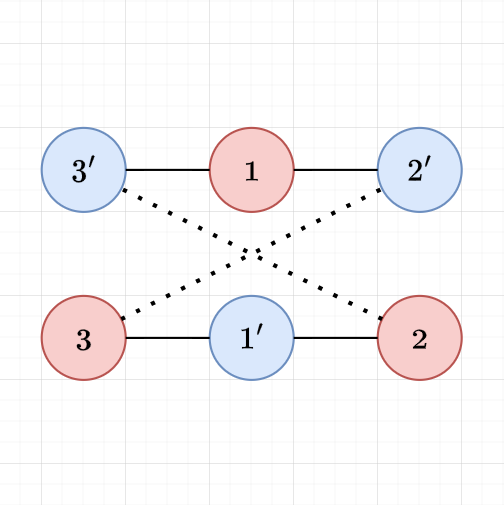
\includegraphics[scale=0.3]{images/not_bipartite.png}
                \end{center}
            \end{column}
        \end{columns}
    \end{frame}

    %LCA
    \section{最低共同祖先}
    \begin{frame}
        \frametitle{甚麼是最低共同祖先?}
        
        \begin{itemize}
            \item 最低共同祖先,又叫 LCA(Lowest Common Ancestor)
            \item 找 $a$ 和 $b$ 的 LCA,如果 $a$ 是 $b$ 的祖先,那 $a$ 就是他們的 LCA
            \item 否則就是找他們兩個的祖先中,深度最深的那個點
        \end{itemize}
    \end{frame}
    \begin{frame}{甚麼是最低共同祖先?}
        \begin{center}
            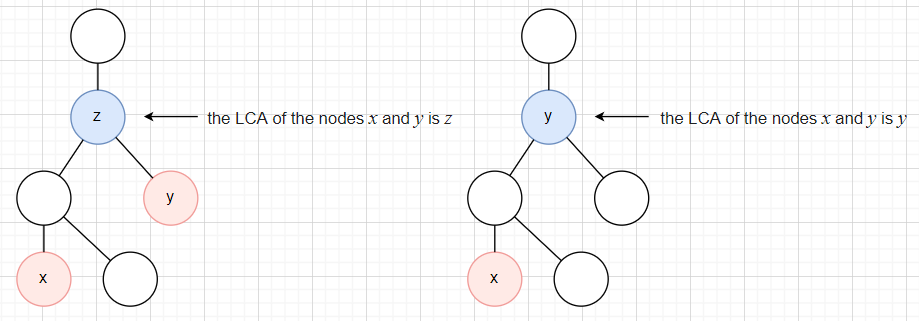
\includegraphics[scale=0.7]{images/what_is_LCA.png}
        \end{center}
    \end{frame}
    \begin{frame}{最低共同祖先}
        \begin{itemize}
            \item 很簡單 R
            \item 就一步一步走嘛
            \item 樹上走路誰不會 R
            \item<2-> 對 R...好水喔 ~ 然後你就 TLE 了
        \end{itemize}
    \end{frame}
    
    \begin{frame}{最低共同祖先}
        \begin{itemize}
            \item 剛剛一步一步往上走的方式太慢了
            \item 最糟的狀況下,我們從根開始,會往上走整棵樹的高度欸 QwQ
            \item<2-> 所以你不能用走的,要用跳的
            \item<2-> 有一個東西叫\textbf{倍增法}
        \end{itemize}
    \end{frame}
    
    \begin{frame}{倍增法往上跳}
        \begin{columns}
            \begin{column}{0.65 \textwidth}
                \begin{itemize}
                    \item 我們用二進位的概念來想
                    \item 對每個點 $u$ 開一個陣列 $p[i][u]$,代表從點 $u$ 往上跳 $2^i$ 條邊會到的節點
                \end{itemize}
            \end{column}
            \begin{column}{0.4 \textwidth}
                \begin{center}
                    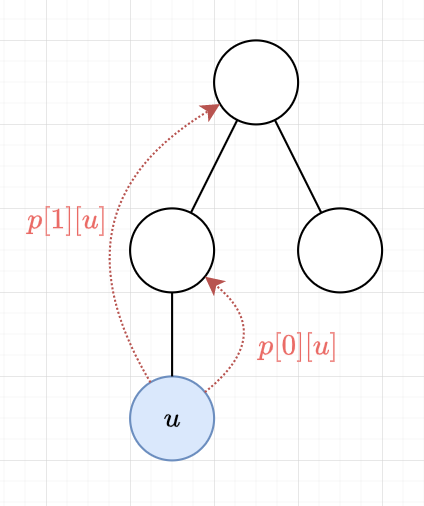
\includegraphics[scale=0.3]{images/binary_lifting.png}
                \end{center}
            \end{column}
        \end{columns}
    \end{frame}
    
    \begin{frame}{倍增法往上跳}
        \begin{columns}
            \begin{column}{0.65 \textwidth}
                \begin{itemize}
                    \item 要計算這個,我們可以枚舉  $i = 0 \sim \lfloor \log_2 n \rfloor$
                    \item 依序去轉移每個點往上跳的答案
                    \item 轉移式:$p[i][u] = p[i-1][p[i-1][u]]$
                    \item $u$ 往上跳 $2^i$ 會是 $u$ 往上跳 $2^{i-1}$ 再往上跳 $2^{i-1}$
                \end{itemize}
            \end{column}
            \begin{column}{0.4 \textwidth}
                \begin{center}
                    \includegraphics[scale=0.3]{images/binary_lifting_transition.png}
                \end{center}
            \end{column}
        \end{columns}
    \end{frame}
    
    \begin{frame}{倍增法找 LCA}
        \begin{itemize}
            \item 有了剛剛的表,現在來找 $a$ 和 $b$ 的 LCA owo
            \item 想法是我們可以把 $a$ 往上跳
            \item 既然要知道 $a,b$ 兩個人的 LCA
            \item 那其實我們只要一路去判斷 $a$ 的祖先 $v$ 是不是 $b$ 的祖先就好了
            \item 判斷祖先可以用剛剛講到的樹壓平來處理 ><
        \end{itemize}
    \end{frame}
    
    \begin{frame}{倍增法找 LCA}
        \begin{columns}
            \begin{column}{0.65 \textwidth}
                \begin{itemize}
                    \item 只要 $a$ 往上跳 $2^i$ 格不是 $b$ 的祖先,就一直往上跳
                    \item 之後 LCA 就會是 $p[0][a]$ 了
                    \item<2-> 預處理$O(n \log n)$、單筆詢問$O(\log n)$
                \end{itemize}
            \end{column}
            \begin{column}{0.4 \textwidth}
                \begin{center}
                    \includegraphics[scale=0.25]{images/binary_lifting_lca.png}
                \end{center}
            \end{column}
        \end{columns}
    \end{frame}
    
    \begin{frame}{倍增法找 LCA}
        \begin{columns}
            \begin{column}{0.65 \textwidth}
                \begin{itemize}
                    \item 有另一種寫法
                    \item<2-> 我們先把 $a$和$b$拉到同一個高度
                    \item<2-> 讓$a$和$b$同時一起往上跳
                    \item<2-> 只要不會是同個點就往上跳
                    \item<3-> 最後我們會找到的點 $v$ 是他們 LCA 的子節點
                    \item<3-> 所以 LCA 是 $v$ 的父節點 $dp[0][v]$
                \end{itemize}
            \end{column}
            \begin{column}{0.4 \textwidth}
                \begin{center}
                    \includegraphics[scale=0.3]{images/binary_lifting_lca_2.png}
                \end{center}
            \end{column}
        \end{columns}
    \end{frame}
    
    \begin{frame}{倍增法找 LCA}
        \begin{itemize}
            \item 有第三種寫法和第四種寫法
            \item<2-> 樹壓平 + RMQ 或 輕重鍊剖分 (HLD)
            \item<2-> 這些東西今天不會講,因為會用到資料結構的東西
            \item<2-> 有興趣的自己上網查 XD
        \end{itemize}
    \end{frame}
    \begin{frame}{喵喵喵喵喵}
        \begin{center}
            現在來看一些可以寫的例題 ><
        \end{center}
    \end{frame}
    
    \begin{frame}
        \frametitle{這是一題很裸很裸的題目 ><}
        \begin{block}{\href{https://cses.fi/problemset/task/1688/}{CSES Company Queries II}}
        找 LCA
        \end{block}
    \end{frame}
    
    \begin{frame}
        \frametitle{樹上兩點距離}
        \begin{block}{\href{https://tioj.ck.tp.edu.tw/problems/2172}{TIOJ 2172 物種演化 (Evolution)}}
        給你一棵樹,接下來詢問 $a,b$ 的距離
        \end{block}
        
        \begin{itemize}
            \item<2-> 兩點的距離其實就是 $dep[a] + dep[b] - 2 \cdot dep[lca(a,b)]$
        \end{itemize}
    \end{frame}
    %MST
    \section{最小生成樹}
    \begin{frame}
        \frametitle{甚麼是最小生成樹?}
        \begin{itemize}
            \item 最小生成樹,又叫 MST(Minimum Spanning Tree)
            \item 給你一張圖,從圖上找一些邊,讓它是一棵樹並且使邊權總合最小
            \item 可能不唯一
            \item 兩種演算法:Kruskal's Algorithm、Prim's Algorithm
        \end{itemize}
    \end{frame}
    
    \begin{frame}
        \frametitle{最小生成樹}
        \begin{center}
            \includegraphics[scale=0.45]{images/mst.png}
        \end{center}
    \end{frame}
    
    
    \begin{frame}
        \frametitle{Kruskal's Algorithm}
        \begin{itemize}
            \item 把邊權由小排到大
            \item 從最小的開始,把該條邊加進樹
            \item 並查集維護:如果邊所連接的兩點祖先相同,就會產生環
            \item 如果會形成環,就略過它
            \item 它算是一種 greedy
            \item 時間複雜度 $O(|E| \log|E|)$
        \end{itemize}
    \end{frame}
    
    \begin{frame}
        \frametitle{Kruskal's Algorithm}
        \begin{columns}
            \begin{column}{0.5 \textwidth}
                \begin{center}
                    \includegraphics[scale=0.4]{images/mst_example.png}
                \end{center}
            \end{column}
            \begin{column}{0.5 \textwidth}
                \texttt{Sorted Edges:} \\
                \texttt{\{1,2\}, \{1,5\}, \{4,5\}, \{1,4\}} \\ 
                \texttt{\{1,3\}, \{2,4\}, \{3,4\}, \{2,3\}}
                \begin{enumerate}
                    \item add \texttt{\{1,2\}}
                    \item add \texttt{\{1,5\}}
                    \item add \texttt{\{4,5\}}
                    \item \sout{add \texttt{\{1,4\}}} (cycle!)
                    \item add \texttt{\{1,3\}}
                    \item \sout{add \texttt{\{2,4\}}} (cycle!)
                    \item \sout{add \texttt{\{3,4\}}} (cycle!)
                    \item \sout{add \texttt{\{2,3\}}} (cycle!)
                \end{enumerate}
            \end{column}
        \end{columns}
    \end{frame}
    
    \begin{frame}
        \frametitle{Kruskal's Algorithm 證明}
        令 Kruskal 算法得出的生成樹為 $K$,另一棵生成樹為 $T$。\\
        按照 Kruskal 算法加邊的順序,找到第一條不在 $T
        $裡的邊 $e_1$,把 $e_1$ 加到 $T$ 裡必定會形成環,環上必定會有一條不在 $K$ 中的邊 $e_2$(一定只有一條),因為 Kruskal 算法先選了 $e_1$,代表 $w(e_1) \leq w(e_2)$。\\
        然後再把 $e_2$ 拔掉,可以得到權重比原本的 $T$ 還要小的生成樹,所以一直重複上述動作,就可以把$T$ 中權重較大的邊替換掉,最後$T$就會$=K$,$K$ 就會是最小生成樹
        \begin{center}
            \includegraphics[scale=0.27]{images/kruskal_proof.png}
        \end{center}
    \end{frame}
    
    \begin{frame}
        \frametitle{Prim's Algorithm}
        \begin{itemize}
            \item 起點:隨便一個點,然後把它加到樹上
            \item 每次選樹上的所有點連出去的邊中權重最小的
            \item 然後把點跟邊加到樹裡面,最後就會得到 MST
            \item 時間複雜度 $O(|V|+|E| \log|V|)$
            \item 稠密圖可以在 $O(|V|^2)$ 的時間完成,會比 Kruskal 快
        \end{itemize}
    \end{frame}
    
    \begin{frame}
        \frametitle{Prim's Algorithm}
        \begin{columns}
            \begin{column}{0.5 \textwidth}
                \begin{center}
                    \includegraphics[scale=0.4]{images/prim_example.png}
                \end{center}
            \end{column}
            \begin{column}{0.5 \textwidth}
                (pq 按照走到 $u$ 的邊權由小到大排)
                \begin{enumerate}
                    \item \texttt{push} $1$, $\sum w = 0$ , \texttt{pq = \{7,2,3\}}
                    \item \texttt{pop} $7$ , $\sum w = 1$ , \texttt{pq = \{2,3,6\}}
                    \item \texttt{pop} $2$ , $\sum w = 3$ , \texttt{pq = \{3,4,6\}}
                    \item \texttt{pop} $3$ , $\sum w = 6$ , \texttt{pq = \{4,6,5\}}
                    \item \texttt{pop} $4$ , $\sum w = 10$, \texttt{pq = \{6,5\}}
                    \item \texttt{pop} $6$ , $\sum w = 15$, \texttt{pq = \{5\}}
                    \item \texttt{pop} $5$ , $\sum w = 19$
                \end{enumerate}
            \end{column}
        \end{columns}
    \end{frame}
    
    \begin{frame}
        \frametitle{Prim's Algorithm}
        實作細節:
        \begin{itemize}
            \item 與 Dijkstra 的寫法很像
            \item priority queue 存 \{邊權, 點\}
            \item 稠密圖可以直接做 $|V|$ 次,每次枚舉與當前點集相鄰且邊權最小的點
        \end{itemize}
    \end{frame}
    
    \begin{frame}
        \frametitle{Prim's Algorithm 證明}
        證明:走的每一步都在 MST 中\\
        假設第$k$步成立,這個時候的邊集為$E$,且包含在 MST 中 \\
        令 MST 為$T$,接下來要加入的邊為$e_1$。\\
        \begin{enumerate}
            \item 如果$e_1$在 $T$ 中,那就會成立。
            \item 否則將$e_1$加入 $T$ 中,加入後必定會形成環,環上必定有一條不在$E$中的邊$e_2$。
        \end{enumerate}
        $e_1$ 不可能大於 $e_2$,因為算法先選了 $e_1$。\\
        $e_1$ 不可能小於 $e_2$,因為如果 $e_1$ 小於 $e_2$,$T+e_1-e_2$會比 MST 更小。\\
        因此 $e_1=e_2$,$T+e_1-e_2$是 MST,$E$包含在其中。
        \begin{center}
            \includegraphics[scale=0.16]{images/prim_proof.png}
        \end{center}
    \end{frame}
    \begin{frame}
        \frametitle{練習}
        \begin{block}{\href{https://cses.fi/problemset/task/1675}{CSES Road Reparation}}
        找最小生成樹
        \end{block}
    \end{frame}
    \begin{frame}
        \frametitle{Cycle Property}
        \begin{itemize}
            \item 定義:\\
            假設$T$是一個帶權的最小生成樹,加入一條邊不在 $T$ 上的邊$e$以後,則會形成一個環,並且$e$會比環上任一條邊的邊權都大。($T$ 一定不會選環上權重最大的邊)
            \item 證明:\\
            我們可以利用反證法,如果環上存在一條邊$d$比$e$大,那我們可以把$d$拔掉,換成$e$,那麼這樣得到的生成樹會比$T$還要小,矛盾。
        \end{itemize}
    \end{frame}
    \begin{frame}
        \frametitle{Cut Property}
        \begin{itemize}
            \item 定義:\\
            若將圖$G$分成兩個連通塊,那我們找到的最小生成樹中,必存在一條連接兩個連通塊的邊,而且這條邊是所有可以連接兩個連通塊的邊中最小的。($T$ 一定會選割上權重最小的邊)
            \item 證明:\\
            一樣可以用反證法,我覺得你們可以自己證。
        \end{itemize}
    \end{frame}
    \begin{frame}
        \frametitle{應用}
        \begin{itemize}
            \item 找非嚴格次小生成樹。
            \item<2-> 根據 cycle property 我們可以發現,次小生成樹跟最小生成樹相差一條邊
            \item<3-> 既然我們知道只差一條邊了,假設那條邊連接$u$和$v$,那就枚舉不在 MST 上的邊
            \item<3->讓這些邊去跟在 MST 中$u$到$v$路徑上的邊做替換,替換掉最大的邊最優
        \end{itemize}
        \begin{center}
            \includegraphics[scale=0.3]{images/smst.png}
        \end{center}
    \end{frame}
    
    \begin{frame}
        \frametitle{非嚴格次小生成樹}
        \begin{columns}
            \begin{column}{0.65 \textwidth}
                \begin{itemize}
                    \item 可以用前面講過的倍增法去維護兩點路徑間的最大邊
                    \item 維護一個 $mx[i][u]$ 表示 $u$ 往上跳 $2^i$ 條邊的最大邊
                    \item 在轉移時順便維護這個值
                    \item 轉移式: $$mx[i][u] = \max(mx[i-1][u], mx[i-1][p[i-1][u]])$$
                \end{itemize}
            \end{column}
            \begin{column}{0.4 \textwidth}
                \begin{center}
                    \includegraphics[scale=0.2]{images/find_smst.png}
                \end{center}
            \end{column}
        \end{columns}
    \end{frame}
   
\end{document}